%definira klasu dokumenta 
\documentclass[12pt]{report} 

%prostor izmedu naredbi \documentclass i \begin{document} se zove uvod. U njemu se nalaze naredbe koje se odnose na cijeli dokument

%osnovni LaTex ne može riješiti sve probleme, pa se koriste različiti paketi koji olakšavaju izradu željenog dokumenta
\usepackage[croatian]{babel} 
\usepackage{amssymb}
\usepackage{amsmath}
\usepackage{txfonts}
\usepackage{mathdots}
\usepackage{titlesec}
\usepackage{array}
\usepackage{lastpage}
\usepackage{etoolbox}
\usepackage{longtable, tabu}
\usepackage{color, colortbl}
\usepackage{adjustbox}
\usepackage{geometry}
\usepackage[classicReIm]{kpfonts}
\usepackage{hyperref}
\usepackage{fancyhdr}

\usepackage{float}
\usepackage{setspace}
\restylefloat{table}


\patchcmd{\chapter}{\thispagestyle{plain}}{\thispagestyle{fancy}}{}{} %redefiniranje stila stranice u paketu fancyhdr

%oblik naslova poglavlja
\titleformat{\chapter}{\normalfont\huge\bfseries}{\thechapter.}{20pt}{\Huge}
\titlespacing{\chapter}{0pt}{0pt}{40pt}


\linespread{1.3} %razmak između redaka

\geometry{a4paper, left=1in, top=1in,}  %oblik stranice

\hypersetup{ colorlinks, citecolor=black, filecolor=black, linkcolor=black,	urlcolor=black }   %izgled poveznice


%prored smanjen između redaka u nabrajanjima i popisima
\newenvironment{packed_enum}{
	\begin{enumerate}
		\setlength{\itemsep}{0pt}
		\setlength{\parskip}{0pt}
		\setlength{\parsep}{0pt}
	}{\end{enumerate}}

\newenvironment{packed_item}{
	\begin{itemize}
		\setlength{\itemsep}{0pt}
		\setlength{\parskip}{0pt}
		\setlength{\parsep}{0pt}
	}{\end{itemize}}


%boja za privatni i udaljeni kljuc u tablicama
\definecolor{LightBlue}{rgb}{0.9,0.9,1}
\definecolor{LightGreen}{rgb}{0.9,1,0.9}


%podesavanje zaglavlja i podnožja

\pagestyle{fancy}
\lhead{Programsko inženjerstvo}
\rhead{Šahovski Klub}
\lfoot{MISFLIP}
\cfoot{stranica \thepage/\pageref{LastPage}}
\rfoot{\today}
\renewcommand{\headrulewidth}{0.2pt}
\renewcommand{\footrulewidth}{0.2pt}


\begin{document} 
	
	
	
	\begin{titlepage}
		\begin{center}
			\vspace*{\stretch{1.0}} %u kombinaciji s ostalim \vspace naredbama definira razmak između redaka teksta
			\LARGE Programsko inženjerstvo\\
			\large Ak. god. 2020./2021.\\
			
			\vspace*{\stretch{3.0}}
			
			\huge MISFLIP\\
			\Large Dokumentacija, Rev. \textit{0}\\
			
			\vspace*{\stretch{12.0}}
			\normalsize
			Grupa: \textit{MISFLIP}\\
			Voditelj: \textit{Ivar Cmrečak}\\
			
			
			\vspace*{\stretch{1.0}}
			Datum predaje: \textit{$<$dan$>$. $<$mjesec$>$. $<$godina$>$.}\\
	
			\vspace*{\stretch{4.0}}
			
			Nastavnik: \textit{Igor Stančin}\\
		
		\end{center}

	
	\end{titlepage}

	
	\tableofcontents

	\chapter{Dnevnik promjena dokumentacije}
		
		\textbf{\textit{Kontinuirano osvježavanje}}\\
				
		
		\begin{longtabu} to \textwidth {|X[2, l]|X[13, l]|X[3, l]|X[3, l]|}
			\hline \multicolumn{1}{|l|}{\textbf{Rev.}}	& \multicolumn{1}{l|}{\textbf{Opis promjene/dodatka}} & \multicolumn{1}{|l|}{\textbf{Autori}} & \multicolumn{1}{l|}{\textbf{Datum}} \\[3pt] \hline
			\endfirsthead
			
			\hline \multicolumn{1}{|l|}{\textbf{Rev.}}	& \multicolumn{1}{l|}{\textbf{Opis promjene/dodatka}} & \multicolumn{1}{|l|}{\textbf{Autori}} & \multicolumn{1}{l|}{\textbf{Datum}} \\[3pt] \hline
			\endhead
			
			\hline 
			\endlastfoot
			
			0.1 & Napravljen predložak.	& Klabučar & 08.10.2020. 		\\[3pt] \hline 
			0.2 & Napisani dionici i napravljeni funkcionalni zahtjevi za aktore & Kedmenec & 10.10.2020. 		\\[3pt] \hline 
			0.2.1 & Napisana motivacija za projekt & Klabučar & 12.10.2020. \\[3pt] \hline
			0.2.2 & Napravljene dopune funkcionalnih zahtjeva & Paprskar & 13.10.2020. \\[3pt] \hline
			0.3 & Napisani opisi obrazaca uporabe za neregistriranog korisnika, trenera i članove & Svetec, Klabučar, Paprskar & 19.10.2020. 		\\[3pt] \hline 
			0.3.1 & Napisani opisi obrazaca uporabe za administratora & Kedmenec & 20.10.2020. \\[3pt] \hline
			0.4 & Napisani nefunkcionalni zahtjevi i zahtjevi domene & Kedmenec & 24.10.2020. \\[3pt] \hline
			0.4.1 & Dodani sekvencijski dijagrami za revidiranje taktike i stvaranje treninga & Klabučar & 25.10.2020. \\[3pt] \hline
			0.4.2 & Dodan sekvencijski dijagram za objavu taktike & Leontić & 28.10.2020. \\[3pt] \hline
			0.4.3 & Dodan sekvencijski dijagram za riješavanje taktike & Žižić & 28.10.2020. \\[3pt] \hline
			0.4.4 & Dodan dijagram obrasca uporabe za funkcionalnost trenera & Paprskar & 29.10.2020. \\[3pt] \hline
			0.4.5 & Modificirani obrasci uporabe & Paprskar & 29.10.2020. \\[3pt] \hline
			0.4.6 & Dodan dijagram obrasca uporabe za funkcionalnost neregistriranog korisnika i člana & Svetec & 29.10.2020. \\[3pt] \hline
			0.4.7 & Dodan dijagram obrasca uporabe za funkcionalnost administratora & Cmrečak & 30.10.2020. \\[3pt] \hline
			0.4.8 & Numerirani svi obrasci uporabe i dodan UC19 & Svetec & 2.11.2020. \\[3pt] \hline
			0.4.9 & Dodane tablice vezane uz treninge i turnire & Leontić & 2.11.2020. \\[3pt] \hline
			0.4.10 & Ispravljen dijagram za riješavanje taktike & Žižić & 3.11.2020. \\[3pt] \hline
			0.4.11& Ispravljen dijagram obrasca uporabe za funkcionalnost trenera & Paprskar & 4.11.2020. \\[3pt] \hline
			0.4.12& Dodane tablice baze podatake vezane uz taktike & Klabučar & 5.11.2020. \\[3pt] \hline
			0.5 & Dodan opis projektnog zadatka & Leontić & 5.11.2020 \\[3pt] \hline
			0.5.1 & Ispravljen admin use case dijagram i povezana dokumentacija & Žižić & 5.11.2020. \\[3pt] \hline
			0.5.2 & Dovršen opis projektnog zadatka & Paprskar & 6.11.2020 \\[3pt] \hline
			0.5.3 & Dodana tablica transakcija & Leontić & 6.11.2020 \\[3pt] \hline
			0.5.4 & Dodan dijagram baze podataka & Svetec & 6.11.2020. \\[3pt] \hline
			0.5.5 & Dodani dijagrami razreda & Klabučar & 7.11.2020. \\[3pt] \hline
			0.5.6 & Gramatički ispravljen dio dokumentacije & Paprskar & 9.11.2020. \\[3pt] \hline
			0.5.7 & Ispravljena veza između UC2 i UC3 & Svetec & 10.11.2020. \\[3pt] \hline
			0.5.8 & Dodan opis korištenog susatava baza podataka & Kedmenec & 10.11.2020. \\[3pt] \hline
			0.6 & Popunjena tablica aktivnosti & Paprskar, Klabučar & 12.11.2020. \\[3pt] \hline
			0.6.1 & Dodan opis veza uz tablice za trening, turnir i transakcije & Leontić & 12.11.2020 \\[3pt] \hline
			0.6.2 & Dodana literatura & Kedmenec & 12.11.2020 \\[3pt] \hline
			1.0 & Korigiranje teksta i provjera dokumentacije & Kedmenec, Cmrečak, Svetec, Klabučar, Leontić & 13.11.2020 \\[3pt] \hline
			1.1 & Napravljeni dijagram stanja za neregistriranog korisnika i dijagram aktivnosti za revidiranje dojave o pogrešci na taktici & Paprskar & 13.12.2020.\\[3pt] \hline
		\end{longtabu}
	
	
		\textit{Moraju postojati glavne revizije dokumenata 1.0 i 2.0 na kraju prvog i drugog ciklusa. Između tih revizija mogu postojati manje revizije već prema tome kako se dokument bude nadopunjavao. Očekuje se da nakon svake značajnije promjene (dodatka, izmjene, uklanjanja dijelova teksta i popratnih grafičkih sadržaja) dokumenta se to zabilježi kao revizija. Npr., revizije unutar prvog ciklusa će imati oznake 0.1, 0.2, …, 0.9, 0.10, 0.11.. sve do konačne revizije prvog ciklusa 1.0. U drugom ciklusu se nastavlja s revizijama 1.1, 1.2, itd.}
	\chapter{Opis projektnog zadatka}
		
		 \noindent   Cilj projekta je razvijanje aplikacije za šahovski klub. Aplikacijom će
			se moći služiti:
			
			\begin{description}
				\item[$\bullet$] treneri 
				\item[$\bullet$] članovi
				\item[$\bullet$] neregistrirani korisnici
			\end{description} 
		    Aplikacijom će upravljati administrator. Jedna osoba može imati samo jednu od ove
			četiri uloge. Glavne koristi aplikacije su interaktivno učenje šaha,
			natjecanje protiv drugih članova kluba u turnirima i infomiranje članova
			o aktivnostima i novostima u klubu. Članovi mogu preko aplikacije plaćati članarinu. Korisnici će učiti šah pomoću dnevnih šahovskih
			taktika, koje postavljaju treneri. Treneri mogu organizirati turnire,
			organizirati treninge i informirati članove pomoću stranice s novostima.
			Neregistrirani korisnici imat će ograničene mogućnosti kod korištenja
			aplikacije. \\
		    Korisnik koji prvi puta pokreće aplikaciju i nije registriran smjeti će
			pristupiti novostima i informirati se o svim događanjima u klubu,
			rješavati dnevne šahovske taktike, ali neće biti dio rang lista, na
			kojima će biti popisani najuspješniji članovi koji su rješavali dnevne
			taktike. Status člana potreban je i za pristup organiziranim treninzima
			i turnirima. Ukoliko je korisnik zainteresiran za učlanjenje u klub,
			smjeti će napraviti korisnički račun, za koji su potrebni:
			\begin{description}
			\item[$\bullet$] korisničko ime
			\item[$\bullet$] e-mail
			\item[$\bullet$] lozinka. 
	    	\end{description} 
			Pri izradi računa korisnik se mora složiti s
			pravilima kluba (ne smije varati pomoću \textit{``chess engine''}-a , ne smije
			koristiti tuđi korisnički račun ili dati svoj drugima na korištenje, ne
			smije se neprikladno ponašati prema trenerima ili drugim članovima...).
			Nakon uspješne registracije, kako bi dobio status člana, registrirani
			korisnik mora platiti članarinu. Nakon ispunjavanja formulara u koji se
			upisuju ime i prezime člana, mjesec za koji se članarina plaća, dob,
			broj mobitela i e-mail adresa, ako je transakcija uspješno provedena
			administrator korisniku dodjeljuje status člana. Status člana bit će
			maknut ukoliko korisnik prestane plaćati članarinu, tj. transakcija za
			određeni mjesec ne bude provedena i upisana u bazu podataka. Članovi uz
			rješavanje taktike imaju mogućnost dodijeliti ocjenu taktici ovisno o
			njenoj težini (1-5), a u slučaju da misle da postoji pogreška u taktici
			ili vide bolje rješenje, mogu prijaviti pogrešku. Rang liste za taktike
			rade se ovisno o vremenu koje je članu potrebno da točno riješi taktiku
			i težini taktike. U aplikaciji postoje rang liste koje prikazuju
			najbolje rješavače taktika. Nove rang liste postavljaju se svaki mjesec.
			U taktici je dozvoljen samo jedan poredak poteza, a u slučaju pogrešnog
			poteza rješavaču se dodaje vremenska kazna (1 minuta) za svaki pogrešan
			potez. Ako član misli da je uočio pogrešku u taktici, može je prijaviti
			tako da nakon pritiska na gumb za prijavu pogreške u otvorenu simulaciju
			taktike unese poteze za koje misli da su ispravni i dodatno obrazloži
			poteze u tekstualnoj kućici ako smatra da je potrebno. Ako član želi
			dodatno vježbati, može se prijaviti na organizirani trening kod trenera.
			Trener u opisu treninga navodi što će sve biti uključeno u njegov
			trening. Nakon vježbanja član može testirati svoju vještinu protiv
			drugih igrača u sklopu turnira. Na stranici turnira član može vidjeti
			raspored nadolazećih turnira i prijaviti se ako ima slobodnih mjesta.
			Turniri se održavaju u točno određeno vrijeme. Tada članovi koji su se
			prijavili igraju jedan protiv drugog sve dok se ne proglasi pobjednik
			(igre se ne odvijaju u sklopu aplikacije). Turniri se održavaju u
			različitim formatima:
			\begin{description} 
			\item[$\bullet$] \textit{rapid} (25 minuta po igraču)
		    \item[$\bullet$] \textit{blitz} (5 minuta po igraču)
			\item[$\bullet$] \textit{bullet} (2 minute po igraču)
		    \end{description}
			 Na stranici turnira postavlja se
			očekivano ukupno vrijeme trajanja turnira. Treneri uz mogućnost
			organiziranja treninga i turnira mogu postavljati dnevne taktike ili
			objavljivati zanimljivosti i novosti. Ako član prijavi pogrešku u
			taktici, da bi došlo do promjene taktike, trener ju mora odobriti. Ako
			trener misli da je žalba valjana, on mijenja taktiku i automatski se
			oduzimaju bodovi za članove koji su riješili pogrešnu verziju taktike,
			te se omogućava ponovno rješavanje ispravljene taktike. Najveće ovlasti
			na stranici ima administrator. On smije dodavati bilo kakav sadržaj,
			brisati sadržaj iz svih rubrika i zabraniti pristup bilo kojem članu i
			treneru. Prilikom brisanja sadržaja, on ostaje u bazi podataka, ali se
			ne prikazuje u aplikaciji. Administrator jedini može dodijeliti uloge
			drugim korisnicima. \\
			Postoje aplikacije sa sličnim mogućnostima poput \textit{chess.com} ili \textit{lichess.org}. Tamo
			je moguće napraviti korisnički račun i vježbati na šahovskim taktikama
			na sličan način kao u našoj aplikaciji, ali te stranice nisu toliko
			fokusirane na rad kluba, nego na učenje i igranje šaha. Ovakve stranice
			pružaju razne mogućnosti poput igre jedan na jedan, učenja šahovskih
			otvaranja, igranja protiv \textit{„chess engine``}-a, što naša aplikacija neće
			sadržavati. Naša aplikacija fokusira se na jedan šahovski klub i njegovu
			organizaciju. \\
			
				\begin{figure}[H]
				\centering
				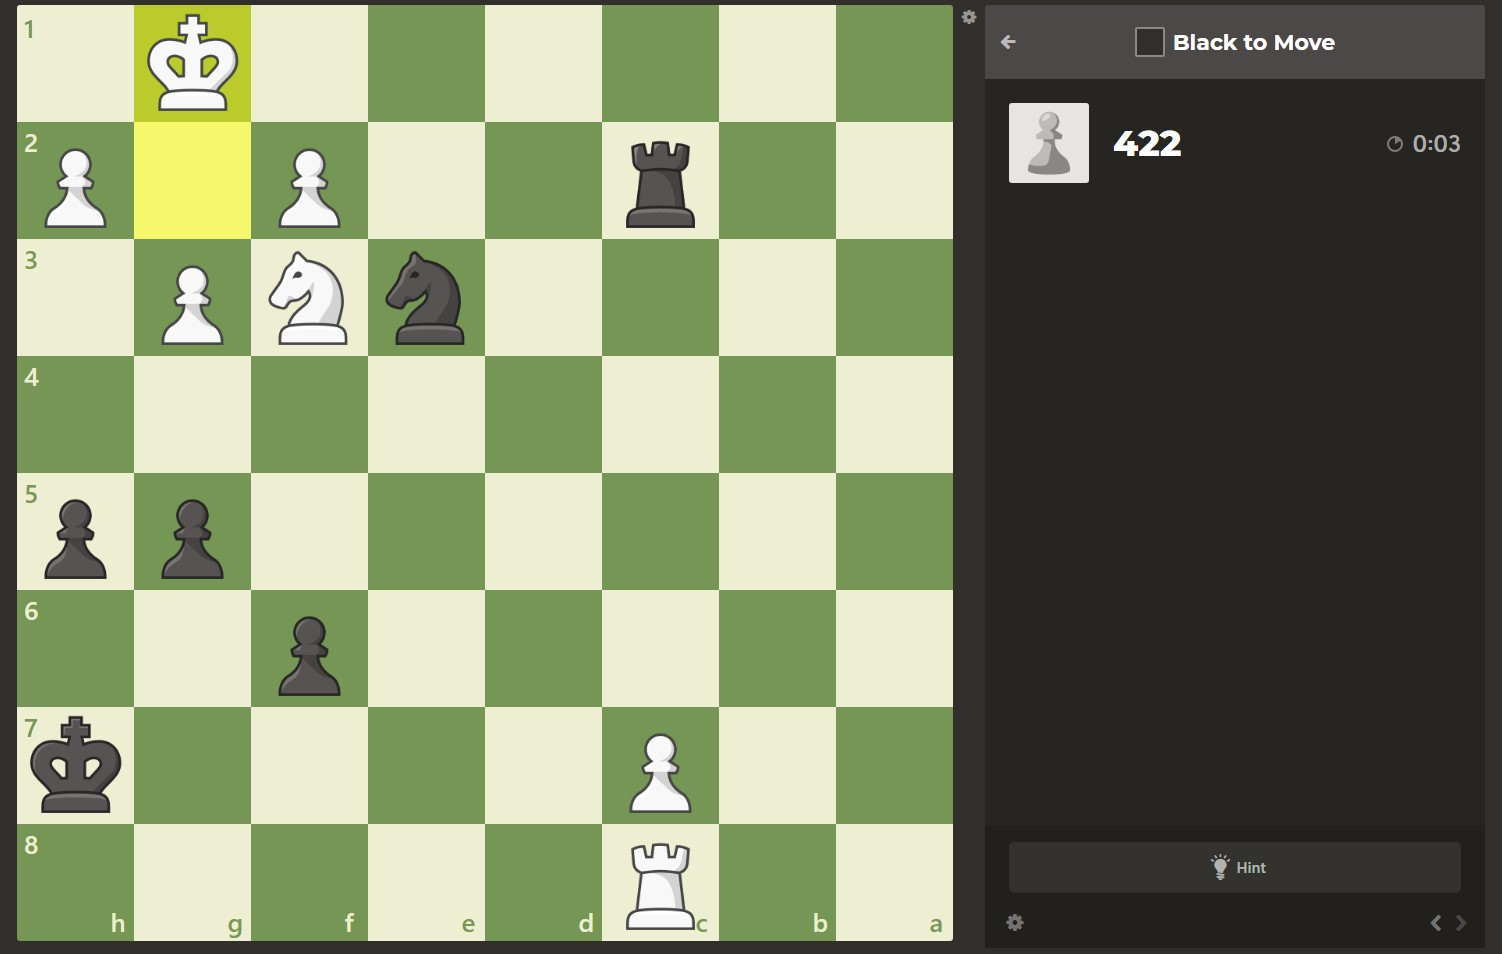
\includegraphics[scale=0.3]{slike/sah-slicno rjesenje.jpeg} %veličina slike u odnosu na originalnu datoteku i pozicija slike
				\caption{Šahovska ploča preuzeta s druge stranice kao primjer drugačijeg rješenja}
				\label{fig:UC$<$broj obrasca$>$}
			\end{figure}
		
	     	\noindent   Za ovakvu aplikaciju mogli bi biti zainteresirani vlasnici šahovskog
			kluba koji žele svojim članovima pružiti više mogućnosti učenja šaha i
			lakši način praćenja novosti u klubu. Postojanje ovakve aplikacije je i
			u interesu svim šahistima koji žele interaktivnije načine sudjelovanja u
			klupskim aktivnostima. Vrlo je vjerojatno da bi šahisti odabrali klub
			koji pruža i online usluge umjesto kluba koji djeluje isključivo uživo. \\
		    Uz sve koristi koje aplikacija pruža, bitno je spomenuti i dosege.
			Projekt omogućava korištenje šahovske ploče za rješavanje dnevnih
			taktika, ali se ne omogućava online igra protiv drugih igrača. Dio
			aplikacije koji se bavi turnirima također ne omogućava 1 na 1 igranje,
			nego samo bilježi raspored turnira i omogućava članovima da se prijave
			na turnir. Organizirani treninzi ne omogućavaju treneru da direktno
			pomoću aplikacije igračima na ploči prikazuje lekcije, nego
			funkcioniraju poput rasporeda gdje članovi mogu vidjeti kada će se
			treninzi održati i kako će izgledati. Dnevne taktike ne omogućavaju
			igračima slobodno postavljanje figurica, nego se koncentriraju na točno
			određenu konfiguraciju ploče. Rješenja dnevnih taktika provjeravaju se
			protiv zadanog slijeda poteza, a ne \textit{``chess engine''}-a (zbog toga se i
			omogućava prijava pogreške u taktici). Prijava pogreške ne sadrži
			dvosmjernu komunikaciju između člana koji se žali i trenera, nego se
			sastoji isključivo od žalbe i mogućeg odobrenja promjene. Aplikacija
			također ne omogućava dvosmjernu komunikaciju (chat) između članova ili
			trenera.\\
			Moguće je nadograditi i proširiti razne aspekte naše aplikacije. Uz
			učenje na dnevnim taktikama moguće je dodati i analiziranje odigranih
			igara ili učenje šahovskih otvaranja. Aplikaciji je moguće dodati neki
			oblik komunikacije između korisnika (forum ili chat). Turniri bi se
			mogli održavati putem aplikacije ako se uz organizacijski aspekt doda i
			mogućnost igranja i bilježenja ratinga, koji bi se računao prema
			uspjehu u igranju protiv drugih članova kluba, a ne samo po uspjehu u
			šahovskim taktikama. Aplikacija bi mogla bilježiti statistike korisnika i
			prikazivati ih na njihovoj osobnoj stranici. Stranici s obavijestima bi
			bilo koristno dodati mogućnost komentiranja na objave. Ukoliko se
			aplikacija želi značajnije proširiti, mogla bi obuhvaćati više šahovskih
			klubova.\\
		    Potencijal za nadogradnju ovog programa u budućnosti svakako bi trebao sadržavati mogućnost testiranja budućih članova i njihovo kategoriziranje u budućem članstvu kluba. To znači da bi budući član osim uplate članarine, koja bi mu omogućila ulaz i korištenje aplikacija šahovskog kluba, trebao proći kroz testne šahovske zadatke koji bi ga prema stupnju uspješnosti stavile u A, B ili C grupu. Primarno grupe ne bi „razbijale“ homogenost šahovskog kluba već bi svakom pojedincu ukazale na stupanj njegovog trenutnog znanja i omogućile kroz treninge i takmičenja njegov rast i napredak. Time bi se statistički moglo pratiti svaki pojedinac. Grupe bi bile određena interna kategorija članova unutar kluba. Samim članovima bio bi izazov pratiti svoju uzlaznu krivulju. \\
		Osim redovne mjesečne članarine trebalo bi omogućiti, kao jednu od budućih nadogradnji kod uplate, opciju da članovi uplaćuju unaprijed za 6 ili 12 mjeseci. Time bi se osim određenih financijskih sredstava koje se korisno mogu utrošiti za razvoj kluba (materijalni i intelektualni troškovi), dobila i jedna stabilna baza igrača na kojoj bi se mogao temeljiti razvoj, ali i opstojnost kluba. Sigurno članstvo osigurava budućnost kluba. Takvim članovima koji se odluče na dugoročnije uplate članarine treba osigurati popuste kod uplate, osigurati određeni reklamni materijal s logom kluba, omogućiti više drugih aktivnosti u samom programu.\\
	    Za pomoć pogledati reference navedene u poglavlju ''Popis literatur'', a po potrebi konzultirati sadržaj na internetu koji nudi dobre smjernice u tom pogledu.
		
		\section{Motivacija za projekt}
		Ideja ovog je projekta olakšati šahovskom klubu obavljanje administrativnih poslova i komunikaciju s članovima. To bi se postiglo web aplikacijom sa funkcionalnostima kao što su online uplaćivanje članarine, objavljivanje novosti, te prijavljivanje članova za treninge i turnire. Web aplikacija bila bi intuitivna i jednostavna za korištenje kako članovima, tako i zaposlenicima kluba. Osim toga, članovi bi se putem web aplikacije mogli nadmetati u rješavanju dnevnih taktika, te tako sudjelovati u šahovskoj zajednici čak i van fizičkog prostora kluba.  \\
Još jedan bitan aspekt ove aplikacije bio bi njen potencijal za nadogradnju. Jasno je da će u budućnosti potrebe šahovskog kluba rasti i da će se trebati uvesti nove funkcionalnosti u web aplikaciju. Tu činjenicu mora odražavati kvaliteta programskog rješenja i dokumentacije kako bi se pružio dobar temelj za nova proširenja.
		
		\eject

		
	
	\chapter{Specifikacija programske potpore}
		
	\section{Funkcionalni zahtjevi}
			
			\textbf{\textit{dio 1. revizije}}\\
			
			\textit{Navesti \textbf{dionike} koji imaju \textbf{interes u ovom sustavu} ili  \textbf{su nositelji odgovornosti}. To su prije svega korisnici, ali i administratori sustava, naručitelji, razvojni tim.}\\
				
			\textit{Navesti \textbf{aktore} koji izravno \textbf{koriste} ili \textbf{komuniciraju sa sustavom}. Oni mogu imati inicijatorsku ulogu, tj. započinju određene procese u sustavu ili samo sudioničku ulogu, tj. obavljaju određeni posao. Za svakog aktora navesti funkcionalne zahtjeve koji se na njega odnose.}\\
			
			
			\noindent \textbf{Dionici:}
			
			\begin{packed_enum}
				
				\item Vlasnik (naručitelj)				
				\item Zaposlenici šahovskog kluba
				\begin{packed_enum}
						
					\item Treneri
						
				\end{packed_enum}
				\item Članovi šahovskog kluba
				\item Neregistrirani korisnici aplikacije
				\item Administrator
				\item Razvojni tim
				
			\end{packed_enum}
			
			\noindent \textbf{Aktori i njihovi funkcionalni zahtjevi:}
			
			
			\begin{packed_enum}
				\item  \underbar{Trener (inicijator) može:}
				
				\begin{packed_enum}
					
					\item prijaviti se u aplikaciju putem korisničkog imena i lozinke
					\item odjaviti se iz aplikacije
					\item postavljati dnevne šahovske taktike
					\item revidirati prijavljenje pogrešne taktike
					\item slagati raspored vlastitih treninga
					\item organizirati turnire
					\item vidjeti rang liste članova
					\item pristupiti i objavljivati novi sadržaj na stranici novosti 
					\item vidjeti osobne podatke i aktivnosti svojeg profila
					
				\end{packed_enum}
			
				\item  \underbar{Član šahovskog kluba (inicijator) može:}
				
				\begin{packed_enum}
					
					\item prijaviti se u aplikaciju putem korisničkog imena i lozinke
					\item odjaviti se iz aplikacije
					\item platiti članarinu putem aplikacije
					\item prijavljivati se na treninge kod pojedinih trenera
					\item prijavljivati se na turnire
					\item rješavati dnevne šahovske taktike
					\begin{packed_enum}
						
						\item nakon rješavanja dnevne šahovske taktike mogu joj dodijeliti ocjenu
						\item nakon rješavanja dnevne šahovske taktike mogu prijaviti grešku u taktici
						
					\end{packed_enum}
					\item vidjeti rang liste članova
					\item pristupiti stranici novosti
					\item vidjeti osobne podatke i aktivnosti svojeg profila
					
				\end{packed_enum}
			
				\item \underbar{Administrator (inicijator) može:}
				
				\begin{packed_enum}
					
					\item prijaviti se u aplikaciju putem korisničkog imena i lozinke
					\item odjaviti se iz aplikacije
					\item potpuno zabraniti pristup bilo kojem članu ili treneru
					\item zabraniti pristup bilo čemu \textbf{osim} uplate članarine bilo kojem članu
					\item vidjeti rang liste članova
					\item objavljivati i skidati sadržaj na stranici novosti
					\item mijenjati raspored treninga bilo kojem treneru
					\item postavljati i skidati dnevne šahovske taktike
					\begin{packed_enum}
						
						\item nakon rješavanja dnevne šahovske taktike mogu joj dodijeliti ocjenu
						\item nakon rješavanja dnevne šahovske taktike mogu prijaviti grešku u taktici
						
					\end{packed_enum}
					\item dodavati i skidati turnire
					\item pregledavati transakcije
					\item vidjeti osobne podatke i aktivnosti svojeg profila
					
				\end{packed_enum}
			
				\item \underbar{Neregistrirani korisnik (inicijator) može:}
				
				\begin{packed_enum}
					
					\item registrirati se
					\item rješavati dnevne šahovske taktike
					\item vidjeti rang liste članova
					\item pristupiti novostima
					
				\end{packed_enum}
			
				\item \underbar{Baza podataka (sudionik):}
				
				\begin{packed_enum}
					
					\item pohranjuje sve podatke o korisnicima i njihovim ovlastima
					\item pohranjuje sve dnevne šahovske taktike
					\item pohranjuje rang listu članova
					\item pohranjuje povijest svih transakcija
					\item pohranjuje termine svih treninga
					\item pohranjuje termine svih turnira
					\item pohranjuje svaku stavku na stranici novosti
					
				\end{packed_enum}
				
			\end{packed_enum}
			
			\eject 
			
			
				
			\subsection{Obrasci uporabe}
				
				\textbf{\textit{dio 1. revizije}}
				
				\subsubsection{Opis obrazaca uporabe}
					\textit{Funkcionalne zahtjeve razraditi u obliku obrazaca uporabe. Svaki obrazac je potrebno razraditi prema donjem predlošku. Ukoliko u nekom koraku može doći do odstupanja, potrebno je to odstupanje opisati i po mogućnosti ponuditi rješenje kojim bi se tijek obrasca vratio na osnovni tijek.}\\
					
					\noindent \underbar{\textbf{UC$<$broj obrasca$>$ - Registracija}}
					\begin{packed_item}
	
						\item \textbf{Glavni sudionik: } Neregistrirani korisnik
						\item  \textbf{Cilj: } Stvoriti korisnički račun za pristup sustavu
						\item  \textbf{Sudionici: } Baza podataka
						\item  \textbf{Preduvjet: } -
						\item  \textbf{Opis osnovnog tijeka:}
						
						\item[] \begin{packed_enum}
	
							\item Korisnik otvara sučelje za registraciju
							\item Korisnik unosi sve potrebne podatke za registraciju
							\item Korisnik prima obavijest o uspješnosti registracije
							
						\end{packed_enum}
						
						\item  \textbf{Opis mogućih odstupanja:}
						
						\item[] \begin{packed_item}
	
							\item[2.a] Unos već postojećeg korisničkog imena i/ili e-maila, unos nepostojećeg e-maila, unos podatka u nedozvoljenom formatu.
							\item[] \begin{packed_enum}
								
								\item Sučelje obavještava korisnika o pogrešci u registraciji i vraća ga na stranicu za registraciju.
								\item Korisnik mijenja podatke i pokušava ponovo ili odustaje od registracije.
								
							\end{packed_enum}
							
						\end{packed_item}
					\end{packed_item}
					

					\noindent \underbar{\textbf{UC$<$broj obrasca$>$ - Pregled dnevnih taktika}}
					\begin{packed_item}
	
						\item \textbf{Glavni sudionik: } Neregistrirani korisnik, član, administrator
						\item  \textbf{Cilj: } Pregledati dostupne taktike za rješavanje tog dana
						\item  \textbf{Sudionici: } Baza podataka
						\item  \textbf{Preduvjet: } -
						\item  \textbf{Opis osnovnog tijeka:}
						
						\item[] \begin{packed_enum}
	
							\item Korisnik otvara stranicu s popisom dnevnih taktika
							\item Korisnik odabire taktiku koju želi rješavati
							\item Pokreće se simulacija šahovske ploče s odabranom taktikom
							
						\end{packed_enum}
					\end{packed_item}


					\noindent \underbar{\textbf{UC$<$broj obrasca$>$ - Rješavanje dnevne taktike}}
					\begin{packed_item}
	
						\item \textbf{Glavni sudionik: } Neregistrirani korisnik, član, administrator
						\item  \textbf{Cilj: } Uspješno riješiti odabranu dnevnu taktiku
						\item  \textbf{Sudionici: }-
						\item  \textbf{Preduvjet: }Korisnik je prethodno odabrao taktiku
						\item  \textbf{Opis osnovnog tijeka:}
						
						\item[] \begin{packed_enum}
	
							\item Korisniku se pokreće simulacija šahovske ploče
							\item Korisnik rješava dnevnu taktiku
							\item Simulacija se zatvara po uspješnom rješavanju
							
						\end{packed_enum}
						
						\item  \textbf{Opis mogućih odstupanja:}
						
						\item[] \begin{packed_item}
	
							
							\item[2.a] Korisnik napravi pogrešan potez
							\item[] \begin{packed_enum}
								
								\item Simulacija obavještava korisnika o pogrešnom potezu i vraća ploču u stanje prije pogrešnog poteza.
								\item Korisnik pokušava s novim potezom.
								
								
							\end{packed_enum}
						
						\item[3.a] Korisnik je prijavljen u aplikaciju kao član
						\item[] \begin{packed_enum}
							
							\item Nakon rješavanja dnevne taktike članu se otvara prozor s mogućnošću davanja ocjene taktici na skali od 1 do 5
							\item Korisnik potvrđuje odabranu ocjenu ili odustaje od davanja ocjene
							\item Članu se otvara prozor s mogućnošću prijave pogreške u taktici
							\item Korisnik u slučaju pogrešaka unosi nove poteze i opis novih poteza
							\item Korisnik potvrđuje unesene informacije ili odustaje od unosa novih poteza i njihovih opisa ako nema pogreške
							
							
						\end{packed_enum}
						\end{packed_item}
					\end{packed_item}


					\noindent \underbar{\textbf{UC$<$broj obrasca$>$ - Pregled rang liste}}
					\begin{packed_item}
	
						\item \textbf{Glavni sudionik: }Korisnik, član, trener, administrator
						\item  \textbf{Cilj: }Pregledati rang listu članova kluba
						\item  \textbf{Sudionici: }Baza podataka
						\item  \textbf{Preduvjet: }Ako je korisnik prijavljen kao član mora imati tekuću članarinu
						\item  \textbf{Opis osnovnog tijeka:}
						
						\item[] \begin{packed_enum}
	
							\item Korisnik otvara stranicu s rang listom
							\item Prikazuje se rang lista članova kluba
							
						\end{packed_enum}
					\end{packed_item}
					

					\noindent \underbar{\textbf{UC$<$broj obrasca$>$ - Pregled novosti}}
					\begin{packed_item}
	
						\item \textbf{Glavni sudionik: }Neregistrirani korisnik, član, trener, administrator
						\item  \textbf{Cilj: }Pregledati novosti
						\item  \textbf{Sudionici: }Baza podataka
						\item  \textbf{Preduvjet: }-
						\item  \textbf{Opis osnovnog tijeka:}
						
						\item[] \begin{packed_enum}
	
							\item Korisnik otvara stranicu s novostima
							\item Korisnik pregledava obajvljene novosti
							
						\end{packed_enum}
					\end{packed_item}
					\eject
					
					\noindent \underbar{\textbf{UC$<$broj obrasca$>$ - Odjava}}
					\begin{packed_item}
	
						\item \textbf{Glavni sudionik: } Administrator, Član, Trener
						\item  \textbf{Cilj: } Okončati aktivnu sjednicu
						\item  \textbf{Sudionici: } Baza podataka
						\item  \textbf{Preduvjet: } Prijava u sustav
						\item  \textbf{Opis osnovnog tijeka:}
						
						\item[] \begin{packed_enum}
	
							\item Klik na gumb 'Odjavi se'
							\item Učitavanje stranice novosti 
							
						\end{packed_enum}
					\end{packed_item}
					
					\noindent \underbar{\textbf{UC$<$broj obrasca$>$ - Objava dnevne šahovske taktike}}
					\begin{packed_item}
	
						\item \textbf{Glavni sudionik: }Trener, administrator
						\item  \textbf{Cilj: } Stvoriti novu dnevnu šahovsku taktiku
						\item  \textbf{Sudionici: } Baza podataka
						\item  \textbf{Preduvjet: } -
						\item  \textbf{Opis osnovnog tijeka:}
						
						\item[] \begin{packed_enum}
	
							\item Otvaranje stranice za unos nove taktike
							\item Trener unosi podatke o taktici poput imena, težine itd.
							\item Trener namješta inicijalnu kofiguraciju ploče na interaktivnoj simulaciji
							\item Trener potvrđuje inicijalnu kofiguraciju
							\item Trener naizmjence pomiče crne i bijele šahovske figurice i tako unosi poteze taktike
							\item Trener potvrđuje korektan unos poteza i objavljuje dnevnu taktiku
							
						\end{packed_enum}
						
						\item  \textbf{Opis mogućih odstupanja:}
						
						\item[] \begin{packed_item}
	
							\item Zabuna u namještanju inicijalne konfiguracije ploče
							\item[] \begin{packed_enum}
								
								\item klik na gumb 'reset'
								\item ploča se vraća na startnu konfiguraciju
								
							\end{packed_enum}
							
							\item Zabuna u unosu poteza taktike
							\item[] \begin{packed_enum}
								
								\item klik na gumb 'reset'
								\item ploča se vraća na inicijalnu konfiguraciju unesenu u prošlom koraku
								
							\end{packed_enum}
							
						\end{packed_item}
					\end{packed_item}
					
					\noindent \underbar{\textbf{UC$<$broj obrasca$>$ - Pregled vlastitih treninga}}
					\begin{packed_item}
	
						\item \textbf{Glavni sudionik: }Trener
						\item  \textbf{Cilj: } Prikazati sve buduće treninge prijavljenog trenera
						\item  \textbf{Sudionici: } Baza podataka
						\item  \textbf{Preduvjet: } -
						\item  \textbf{Opis osnovnog tijeka:}
						
						\item[] \begin{packed_enum}
	
							\item Klik na karticu 'Treninzi'
							\item Kronološki prikaz svih budućih treninga 
						\end{packed_enum}
					\end{packed_item}
					
					
					\noindent \underbar{\textbf{UC$<$broj obrasca$>$ - Brisanje vlastitog treninga}}
					\begin{packed_item}
	
						\item \textbf{Glavni sudionik: }Trener
						\item  \textbf{Cilj: } Obrisati postojeći trening
						\item  \textbf{Sudionici: } Baza podataka
						\item  \textbf{Preduvjet: } Trener se nalazi na stranici pregleda vlastitih treninga
						\item  \textbf{Opis osnovnog tijeka:}
						
						\item[] \begin{packed_enum}
	
							\item klik na gumb za brisanje jednog od prikazanih treninga
							\item prikaz dijaloškog okvira koji traži potvrdu od trenera da uistinu želi obrisati trening
							\item nakon davanja potvrde trening nestaje iz prikaza
							
						\end{packed_enum}
						
						\item  \textbf{Opis mogućih odstupanja:}
						
						\item[] \begin{packed_item}
	
							\item Trener se predomisli o brisanju treninga
							\item[] \begin{packed_enum}
								
								\item pritisak na gumb 'odustani' u dijaloškom okviru za potvrdu
								
							\end{packed_enum}
							
						\end{packed_item}
					\end{packed_item}
					
					
					\noindent \underbar{\textbf{UC$<$broj obrasca$>$ - Stvaranje novog treninga}}
					\begin{packed_item}
	
						\item \textbf{Glavni sudionik: }Trener
						\item  \textbf{Cilj: } Stvoriti novi trening
						\item  \textbf{Sudionici: } Baza podataka
						\item  \textbf{Preduvjet: } Trener se nalazi na stranici pregleda vlastitih treninga
						\item  \textbf{Opis osnovnog tijeka:}
						
						\item[] \begin{packed_enum}
	
							\item klik na gumb za dodavanje novog treninga
							\item prikaz dijaloškog okvira u koji trener unosi podatke o treningu kao vrijeme, naziv itd.
							\item klik na gumb za stvaranje treninga
							\item zatvara se dijaloški okvir i novi trening dodaje se u prikaz treninga
							
						\end{packed_enum}
						
						\item  \textbf{Opis mogućih odstupanja:}
						
						\item[] \begin{packed_item}
	
							\item Odustajanje od stvaranja novog treninga
							\item[] \begin{packed_enum}
								
								\item pritisak na gumb 'odustani' u dijaloškom okviru za unos podataka o treningu
								\item zatvaranje dijaloškog okvira i odbacivanje unesenih podataka
								
							\end{packed_enum}
							
						\end{packed_item}
					\end{packed_item}
					
					\noindent \underbar{\textbf{UC$<$broj obrasca$>$ - Pregled turnira}}
					\begin{packed_item}
	
						\item \textbf{Glavni sudionik: }Trener, Administrator, Član, Korisnik ?
						\item  \textbf{Cilj: } Prikazati sve buduće turnire
						\item  \textbf{Sudionici: } Baza podataka
						\item  \textbf{Preduvjet: } -
						\item  \textbf{Opis osnovnog tijeka:}
						
						\item[] \begin{packed_enum}
	
							\item Klik na karticu 'Turniri'
							\item Kronološki prikaz svih budućih turnira
						\end{packed_enum}
					\end{packed_item}
					
					\noindent \underbar{\textbf{UC$<$broj obrasca$>$ - Brisanje vlastitog turnira}}
					\begin{packed_item}
	
						\item \textbf{Glavni sudionik: }Trener
						\item  \textbf{Cilj: } Obrisati postojeći turnir čiji je organizator prijavljeni trener
						\item  \textbf{Sudionici: } Baza podataka
						\item  \textbf{Preduvjet: } Trener se nalazi na stranici pregleda turnira, te je vlasnik turnira odabranog za brisanje
						\item  \textbf{Opis osnovnog tijeka:}
						
						\item[] \begin{packed_enum}
	
							\item klik na gumb za brisanje jednog od prikazanih turnira
							\item prikaz dijaloškog okvira koji traži potvrdu od trenera da uistinu želi obrisati turnir
							\item nakon davanja potvrde turnir nestaje iz prikaza
							
						\end{packed_enum}
						
						\item  \textbf{Opis mogućih odstupanja:}
						
						\item[] \begin{packed_item}
	
							\item Trener se predomisli o brisanju turnira
							\item[] \begin{packed_enum}
								
								\item pritisak na gumb 'odustani' u dijaloškom okviru za potvrdu
								
							\end{packed_enum}
							
						\end{packed_item}
					\end{packed_item}
					
					\noindent \underbar{\textbf{UC$<$broj obrasca$>$ - Stvaranje novog turnira}}
					\begin{packed_item}
	
						\item \textbf{Glavni sudionik: }Trener, Administrator
						\item  \textbf{Cilj: } Stvoriti novi turnir
						\item  \textbf{Sudionici: } Baza podataka
						\item  \textbf{Preduvjet: } Trener se nalazi na stranici pregleda turnira
						\item  \textbf{Opis osnovnog tijeka:}
						
						\item[] \begin{packed_enum}
	
							\item klik na gumb za dodavanje novog turnira
							\item prikaz dijaloškog okvira u koji trener unosi podatke o turniru kao vrijeme, naziv itd.
							\item klik na gumb za stvaranje turnira
							\item zatvara se dijaloški okvir i novi turnir dodaje se na stranicu
							
						\end{packed_enum}
						
						\item  \textbf{Opis mogućih odstupanja:}
						
						\item[] \begin{packed_item}
	
							\item Odustajanje od stvaranja novog turnira
							\item[] \begin{packed_enum}
								
								\item pritisak na gumb 'odustani' u dijaloškom okviru za unos podataka
								\item zatvaranje dijaloškog okvira i odbacivanje unesenih podataka
								
							\end{packed_enum}
							
						\end{packed_item}
					\end{packed_item}
					
					\noindent \underbar{\textbf{UC$<$broj obrasca$>$ - Pristup stranici novosti}}
					\begin{packed_item}
	
						\item \textbf{Glavni sudionik: }Član, Trener, Administrator, Neregistrirani korisnik
						\item  \textbf{Cilj: } Vidjeti sve nedavne novosti
						\item  \textbf{Sudionici: } Baza podataka
						\item  \textbf{Preduvjet: } -
						\item  \textbf{Opis osnovnog tijeka:}
						
						\item[] \begin{packed_enum}
	
							\item klik na karticu 'novosti'
							\item prikaz svih nedavnih novosti
							
						\end{packed_enum}
						
					\end{packed_item}
					
					\noindent \underbar{\textbf{UC$<$broj obrasca$>$ - Objava novosti}}
					\begin{packed_item}
	
						\item \textbf{Glavni sudionik: }Trener, Administrator
						\item  \textbf{Cilj: } Objaviti novost na stranici novosti
						\item  \textbf{Sudionici: } Baza podataka
						\item  \textbf{Preduvjet: } Trener se nalazi na stranici novosti
						\item  \textbf{Opis osnovnog tijeka:}
						
						\item[] \begin{packed_enum}
	
							\item klik na gumb za objavu novosti
							\item ispunjavanje dijaloškog okvira za stvaranje novosti
							\item klik na gumb za objavu
							\item novost se prikazuje na vrhu stranice novosti
							
						\end{packed_enum}
						
						\item  \textbf{Opis mogućih odstupanja:}
						
						\item[] \begin{packed_item}
	
							\item Odustajanje od stvaranja novosti
							\item[] \begin{packed_enum}
								
								\item pritisak na gumb 'odustani' u dijaloškom okviru za unos podataka
								\item zatvaranje dijaloškog okvira i odbacivanje unesenih podataka
								
							\end{packed_enum}
							
						\end{packed_item}
					\end{packed_item}
					
					\noindent \underbar{\textbf{UC$<$broj obrasca$>$ - Revidiranje pogreške u taktici}}
					\begin{packed_item}
	
						\item \textbf{Glavni sudionik: }Trener
						\item  \textbf{Cilj: } Prihvatiti ili odbaciti dojavu o pogrešci u nekoj taktici
						\item  \textbf{Sudionici: } Baza podataka
						\item  \textbf{Preduvjet: } Član je prijavio pogrešku u taktici
						\item  \textbf{Opis osnovnog tijeka:}
						
						\item[] \begin{packed_enum}
	
							\item otvara se pregled sa detaljima o dojavi pogreške na taktici
							\item Trener klikom na gumb potvrđuje da je dojava o pogrešci valjana
							\item taktika u pitanju automatski se revidira te se ažuriraju i rang liste članova
							
						\end{packed_enum}
						
						\item  \textbf{Opis mogućih odstupanja:}
						
						\item[] \begin{packed_item}
	
							\item Odbijanje dojave
							\item[] \begin{packed_enum}
								
								\item pritisakom na gumb 'odbaci' dojava se zanemaruje
								
							\end{packed_enum}
							
							
						\end{packed_item}
					\end{packed_item}
					
					\noindent \underbar{\textbf{UC$<$broj obrasca$>$ - Pregled profila}}
					\begin{packed_item}
	
						\item \textbf{Glavni sudionik: }Administrator, Član, Trener
						\item  \textbf{Cilj: } pregled informacija vlastitog profila
						\item  \textbf{Sudionici: } Baza podataka
						\item  \textbf{Preduvjet: } -
						\item  \textbf{Opis osnovnog tijeka:}
						
						\item[] \begin{packed_enum}
	
							\item klik na karticu 'profil'
							\item učitava se prikaz osobnih podataka i svih aktivnosti na aplikaciji
							
						\end{packed_enum}
					\end{packed_item}
					

						\noindent \underbar{\textbf{UC$<$broj obrasca$>$ - Prijava u korisnički račun}}
					\begin{packed_item}
						
						\item \textbf{Glavni sudionik: } Član, trener, administrator
						\item  \textbf{Cilj: } Prijaviti se u korisnički račun
						\item  \textbf{Sudionici: } Baza podataka
						\item  \textbf{Preduvjet: } -
						\item  \textbf{Opis osnovnog tijeka:}
						
						\item[] \begin{packed_enum}
							
							\item Korisnik otvara sučelje za prijavu u korisnički račun
							\item Korisnik upisuje korisničko ime i lozinku
							\item Korisniku se otvara stranica s novostima
							
						\end{packed_enum}
						
						\item  \textbf{Opis mogućih odstupanja:}
						
						\item[] \begin{packed_item}
							
							\item[3.a] Korisnik koji ima status člana nema plaćenu članarinu
							\item[] \begin{packed_enum}
								
								\item Korisniku se otvara stranica za uplatu članarine
								
							\end{packed_enum}
							
						\end{packed_item}
					\end{packed_item}
				
					\noindent \underbar{\textbf{UC$<$broj obrasca$>$ - Uplata članarine}}
				\begin{packed_item}
					
					\item \textbf{Glavni sudionik: }Član
					\item  \textbf{Cilj: } Uplatiti članarinu
					\item  \textbf{Sudionici: } Baza podataka
					\item  \textbf{Preduvjet: } Član je prijavljen u korisnički račun
					\item  \textbf{Opis osnovnog tijeka:}
					
					\item[] \begin{packed_enum}
						
						\item Član odabire opciju "Uplata članarine"
						\item Članu se otvara sučelje s mogućnošću upisa potrebnih podataka za uplatu članarine  
						\item Član upisuje potrebne podatke za uplatu i potvrđuje svoj unos
						\item Član dobiva obavijest da je transakcija uspješna
						
					\end{packed_enum}
					
					\item  \textbf{Opis mogućih odstupanja:}
					
					\item[] \begin{packed_item}
						
					\item[3.a] Član je unio netočne podatke
					\item[] \begin{packed_enum}
						
						\item Članu dolazi obavijest o netočnom unosu podataka te mu se omogućuje da ponovno unese podatke
						
					\end{packed_enum}
						
					\end{packed_item}
				\end{packed_item}
			
			\noindent \underbar{\textbf{UC$<$broj obrasca$>$ - Prijava na trening}}
			\begin{packed_item}
				
				\item \textbf{Glavni sudionik: } Član
				\item  \textbf{Cilj: } Prijaviti se na trening kod odabranog trenera
				\item  \textbf{Sudionici: } Baza podataka
				\item  \textbf{Preduvjet: } Član je prijavljen u korisnički račun i ima tekuću članarinu
				\item  \textbf{Opis osnovnog tijeka:}
				
				\item[] \begin{packed_enum}
					
					\item Član odabire opciju "Prijavite trening"
					\item Članu se prikazuje popis raspoloživih trenera
					\item Član odabire jednog od ponuđenih trenera
					\item Član odabire jedan od raspoloživih termina treninga
					\item Član dobiva obavijest da je željeni termin treninga kod odabranog trenera zabilježen
					
				\end{packed_enum}
			\end{packed_item}
		
		\noindent \underbar{\textbf{UC$<$broj obrasca$>$ - Prijava na turnir}}
		\begin{packed_item}
			
			\item \textbf{Glavni sudionik: } Član
			\item  \textbf{Cilj: } Prijaviti se na turnir
			\item  \textbf{Sudionici: } Baza podataka
			\item  \textbf{Preduvjet: } Član je prijavljen u korisnički račun i ima tekuću članarinu
			\item  \textbf{Opis osnovnog tijeka:}
			
			\item[] \begin{packed_enum}
				
				\item Član odabire opciju "Prijava na turnir"
				\item Članu se javlja obavijest o terminu sljedećeg turnira te poruka o nužnosti potvrde za prijavu na turnir uz mogućnost odabira opcije "Potvrđujem prijavu" ili opcije "Odustajem od prijave"
				\item Član odabire opciju "Potvrđujem prijavu"
				\item Član dobiva obavijest da je prijava zabilježena
				
			\end{packed_enum}
			
			\item  \textbf{Opis mogućih odstupanja:}
			
			\item[] \begin{packed_item}
				
				\item[2.a] Član odustaje od prijave
				\item[] \begin{packed_enum}
					
					\item Član odabire opciju "Odustajem od prijave"
					
				\end{packed_enum}
				
			\end{packed_item}
		\end{packed_item}
		\eject
	
		\noindent \underbar{\textbf{UC$<$broj obrasca$>$ - Brisanje novosti}}
		\begin{packed_item}
		
			\item \textbf{Glavni sudionik: } Administrator
			\item  \textbf{Cilj: } Obrisati novost s stranice novosti
			\item  \textbf{Sudionici: } Baza podataka
			\item  \textbf{Preduvjet: } Korisnik je prijavljen u administratorski korisnički račun
			\item  \textbf{Opis osnovnog tijeka:}
		
			\item[] \begin{packed_enum}
			
				\item Administrator se postavlja na listu novosti
				\item Administrator bira opciju "Obriši obavijest" pored obavijesti koju želi obrisati
				\item Administrator odabire opciju "Da" u dijaloškom okviru za potvrdu
			\end{packed_enum}
	
			\item  \textbf{Opis mogućih odstupanja:}
		
			\item[] \begin{packed_item}
			
				\item[2.a] Administrator odustaje od brisanja novosti
				\item[] \begin{packed_enum}
				
					\item Administrator odabire opciju "Ne" u dijaloškom okviru za potvrdu
				
				\end{packed_enum}
			\end{packed_item}
	
		\end{packed_item}

		\noindent \underbar{\textbf{UC$<$broj obrasca$>$ - Zabrana pristupa treneru ili članu}}
		\begin{packed_item}
		
			\item \textbf{Glavni sudionik: } Administrator
			\item  \textbf{Cilj: } Zabraniti pristup treneru ili članu
			\item  \textbf{Sudionici: } Baza podataka
			\item  \textbf{Preduvjet: } Korisnik je prijavljen u administratorski korisnički račun
			\item  \textbf{Opis osnovnog tijeka:}
		
			\item[] \begin{packed_enum}
			
				\item Administrator se postavlja na listu registriranih korisnika
				\item Administrator bira opciju "Zabrani pristup svemu" pored člana ili trenera kojem želi zabraniti pristup
				\item Administrator odabire opciju "Da" u dijaloškom okviru za potvrdu
			\end{packed_enum}
		
			\item  \textbf{Opis mogućih odstupanja:}
		
			\item[] \begin{packed_item}
			
				\item[2.a] Administrator odustaje od zabrane pristupa
				\item[] \begin{packed_enum}
				
					\item Administrator odabire opciju "Ne" u dijaloškom okviru za potvrdu
				
				\end{packed_enum}
			\end{packed_item}
		
		\end{packed_item}

		\noindent \underbar{\textbf{UC$<$broj obrasca$>$ - Pregled transakcija}}
		\begin{packed_item}
		
			\item \textbf{Glavni sudionik: } Administrator
			\item  \textbf{Cilj: } Pregledati obavljene transakcije
			\item  \textbf{Sudionici: } Baza podataka
			\item  \textbf{Preduvjet: } Korisnik je prijavljen u administratorski korisnički račun
			\item  \textbf{Opis osnovnog tijeka:}
		
			\item[] \begin{packed_enum}
			
				\item Administrator kilkne na karticu "Transakcije"
				\item Na stranici se prikažu sve transakcije
			\end{packed_enum}
		
		\end{packed_item}

		\noindent \underbar{\textbf{UC$<$broj obrasca$>$ - Zabrana pristupa članu osim plaćanja članarine}}
		\begin{packed_item}
			
			\item \textbf{Glavni sudionik: } Administrator
			\item  \textbf{Cilj: } Zabraniti pristup članu svemu osim plaćanju članarine
			\item  \textbf{Sudionici: } Baza podataka
			\item  \textbf{Preduvjet: } Korisnik je prijavljen u administratorski korisnički račun
			\item  \textbf{Opis osnovnog tijeka:}
			
			\item[] \begin{packed_enum}
				
				\item Administrator se postavlja na listu registriranih korisnika
				\item Administrator bira opciju "Zabrani pristup svemu osim plaćanju članarine" pored člana kojem želi zabraniti pristup
				\item Administrator odabire opciju "Da" u dijaloškom okviru za potvrdu
			\end{packed_enum}
			
			\item  \textbf{Opis mogućih odstupanja:}
			
			\item[] \begin{packed_item}
				
				\item[2.a] Administrator odustaje od zabrane pristupa svemu osim plaćanju članarine
				\item[] \begin{packed_enum}
					
					\item Administrator odabire opciju "Ne" u dijaloškom okviru za potvrdu
					
				\end{packed_enum}
			\end{packed_item}
			
		\end{packed_item}
		
		\noindent \underbar{\textbf{UC$<$broj obrasca$>$ - Brisanje treninga}}
		\begin{packed_item}
			
			\item \textbf{Glavni sudionik: } Administrator
			\item  \textbf{Cilj: } Obrisati trening
			\item  \textbf{Sudionici: } Baza podataka
			\item  \textbf{Preduvjet: } Korisnik je prijavljen u administratorski korisnički račun
			\item  \textbf{Opis osnovnog tijeka:}
			
			\item[] \begin{packed_enum}
				
				\item Administrator se postavlja na listu zakazanih treninga
				\item Administrator bira opciju "Obriši trening" pored treninga kojeg želi izbrisati
				\item Administrator odabire opciju "Da" u dijaloškom okviru za potvrdu
			\end{packed_enum}
			
			\item  \textbf{Opis mogućih odstupanja:}
			
			\item[] \begin{packed_item}
				
				\item[2.a] Administrator odustaje od brisanja treninga
				\item[] \begin{packed_enum}
					
					\item Administrator odabire opciju "Ne" u dijaloškom okviru za potvrdu
					
				\end{packed_enum}
			\end{packed_item}
			
		\end{packed_item}
	
		\noindent \underbar{\textbf{UC$<$broj obrasca$>$ - Dodavanje treninga}}
		\begin{packed_item}
			
			\item \textbf{Glavni sudionik: } Administrator
			\item  \textbf{Cilj: } Dodati termin treninga jednome od trenera
			\item  \textbf{Sudionici: } Baza podataka
			\item  \textbf{Preduvjet: } Korisnik je prijavljen u administratorski korisnički račun
			\item  \textbf{Opis osnovnog tijeka:}
			
			\item[] \begin{packed_enum}
				
				\item Administrator se postavlja na listu zakazanih treninga
				\item Administrator bira opciju "Dodaj novi trening"
				\item Otvara se novi dijaloški okvir s poljima za unos podataka te opcijama "Dodaj" i "Odustani"
				\item Administrator unosi podatke o treningu u dijaloški okvir te trenera koji će ga održavati te odabire opciju "Dodaj"
				\item Zatvara se dijaloški okvir i novi trening se dodaje u prikaz treninga
			\end{packed_enum}
			
			\item  \textbf{Opis mogućih odstupanja:}
			
			\item[] \begin{packed_item}
				
				\item[3.a] Administrator odustaje od dodavanja novog treninga
				\item[] \begin{packed_enum}
					
					\item Administrator odabire opciju "Odustani" u dijaloškom okviru za unos podataka o treningu
					
				\end{packed_enum}
				\item[3.b] Uneseni podatci o treningu nisu važeći
				\item[] \begin{packed_enum}
					
					\item Dijaloški okvir se ne zatvori, nego javlja grešku
					
				\end{packed_enum}
			\end{packed_item}
			
		\end{packed_item}
	
		\noindent \underbar{\textbf{UC$<$broj obrasca$>$ - Dodavanje turnira}}
		\begin{packed_item}
			
			\item \textbf{Glavni sudionik: } Administrator
			\item  \textbf{Cilj: } Dodati turnir
			\item  \textbf{Sudionici: } Baza podataka
			\item  \textbf{Preduvjet: } Korisnik je prijavljen u administratorski korisnički račun
			\item  \textbf{Opis osnovnog tijeka:}
			
			\item[] \begin{packed_enum}
				
				\item Administrator se postavlja na listu zakazanih turnira
				\item Administrator bira opciju "Dodaj novi turnir"
				\item Otvara se novi dijaloški okvir s poljima za unos podataka te opcijama "Dodaj" i "Odustani"
				\item Administrator unosi podatke o turniru u dijaloški okvir te odabire trenera kojeg će se smatrati organizatorom tog turnira te odabire opciju "Dodaj"
				\item Zatvara se dijaloški okvir i novi turnir se dodaje u prikaz turnira
			\end{packed_enum}
			
			\item  \textbf{Opis mogućih odstupanja:}
			
			\item[] \begin{packed_item}
				
				\item[3.a] Administrator odustaje od dodavanja novog turnira
				\item[] \begin{packed_enum}
					
					\item Administrator odabire opciju "Odustani" u dijaloškom okviru za unos podataka o turniru
					
				\end{packed_enum}
				\item[3.b] Uneseni podatci o turniru nisu važeći
				\item[] \begin{packed_enum}
					
					\item Dijaloški okvir se ne zatvori, nego javlja grešku
					
				\end{packed_enum}
			\end{packed_item}
			
		\end{packed_item}
		\eject
	
		\noindent \underbar{\textbf{UC$<$broj obrasca$>$ - Brisanje turnira}}
		\begin{packed_item}
			
			\item \textbf{Glavni sudionik: } Administrator
			\item  \textbf{Cilj: } Obrisati turnir
			\item  \textbf{Sudionici: } Baza podataka
			\item  \textbf{Preduvjet: } Korisnik je prijavljen u administratorski korisnički račun
			\item  \textbf{Opis osnovnog tijeka:}
			
			\item[] \begin{packed_enum}
				
				\item Administrator se postavlja na listu zakazanih turnira
				\item Administrator bira opciju "Obriši turnir" pored turnira kojeg želi izbrisati
				\item Administrator odabire opciju "Da" u dijaloškom okviru za potvrdu
			\end{packed_enum}
			
			\item  \textbf{Opis mogućih odstupanja:}
			
			\item[] \begin{packed_item}
				
				\item[2.a] Administrator odustaje od brisanja turnira
				\item[] \begin{packed_enum}
					
					\item Administrator odabire opciju "Ne" u dijaloškom okviru za potvrdu
					
				\end{packed_enum}
			\end{packed_item}
			
		\end{packed_item}
	
		\noindent \underbar{\textbf{UC$<$broj obrasca$>$ - Brisanje dnevne šahovske taktike}}
		\begin{packed_item}
			
			\item \textbf{Glavni sudionik: } Administrator
			\item  \textbf{Cilj: } Obrisati dnevnu šahovsku taktiku
			\item  \textbf{Sudionici: } Baza podataka
			\item  \textbf{Preduvjet: } Korisnik je prijavljen u administratorski korisnički račun
			\item  \textbf{Opis osnovnog tijeka:}
			
			\item[] \begin{packed_enum}
				
				\item Administrator se postavlja na listu dnevnih šahovskih taktika
				\item Administrator bira opciju "Obriši dnevnu šahovsku taktiku" pored dnevne šahovske taktike koju želi izbrisati
				\item Administrator odabire opciju "Da" u dijaloškom okviru za potvrdu
			\end{packed_enum}
			
			\item  \textbf{Opis mogućih odstupanja:}
			
			\item[] \begin{packed_item}
				
				\item[2.a] Administrator odustaje od brisanja dnevne šahovske taktike
				\item[] \begin{packed_enum}
					
					\item Administrator odabire opciju "Ne" u dijaloškom okviru za potvrdu
					
				\end{packed_enum}
			\end{packed_item}
			
		\end{packed_item}
	
		
	
				\subsubsection{Dijagrami obrazaca uporabe}
					
					\textit{Prikazati odnos aktora i obrazaca uporabe odgovarajućim UML dijagramom. Nije nužno nacrtati sve na jednom dijagramu. Modelirati po razinama apstrakcije i skupovima srodnih funkcionalnosti.}
				\eject		
				
								
				
				
			\subsection{Sekvencijski dijagrami}
			
			
				\textbf{Obrazac uporabe UC$<$broj obrasca$>$ - Stvaranje novog treninga}\\
				Trener šalje zahtjev web aplikaciji za stvaranje novog treninga. Web aplikacija dohvaća iz baze podataka sve ostale treninge tog trenera i provjerava da se novi trening ne preklapa ni sa jednim postojećim treningom. Ako uistinu ne postoji preklapanje, novi trening se zapisuje u bazu podataka te se treneru šalje obavijest o uspjehu kreiranja novog treninga. Ukoliko postoji preklapanje s već postojećim treningom, treneru web aplikacija javlja informacije o preklapanju i nemogućnosti stvaranja zatraženog treninga.
				\eject
				
				\makeatletter
                                                                        \newcommand*{\centerfloat}{%
                                                                          \parindent \z@
                                                                          \leftskip \z@ \@plus 1fil \@minus \textwidth
                                                                          \rightskip\leftskip
                                                                          \parfillskip \z@skip}
                                                                   \makeatother
				
				\begin{figure}[H]
					\centerfloat
        					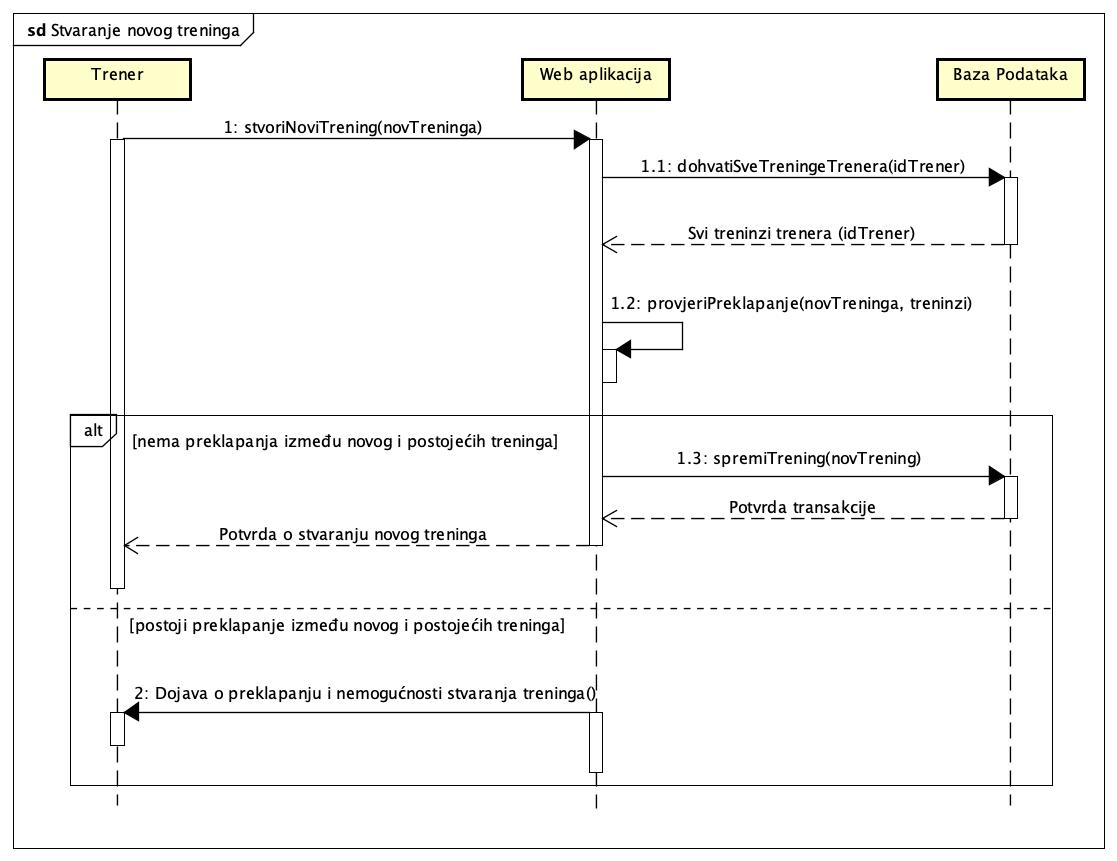
\includegraphics[scale=0.48]{dijagrami/StvaranjeNovogTreninga.jpg} %veličina slike u odnosu na originalnu datoteku i pozicija slike
        					\caption{Sekvencijski dijagram za UC$<$broj obrasca$>$}
        					\label{fig:UC$<$broj obrasca$>$}
				\end{figure}
				
				\eject
				
				\textbf{Obrazac uporabe UC$<$broj obrasca$>$ - Revidiranje pogreške u taktici}\\
				\\Trener šalje zahtjev za prikaz određene dojave o pogrešci taktike kako bi ju mogao pobliže proučiti i odlučiti je li primjedba valjana. Poslužitelj zatraženu dojavu vadi iz baze podataka te ju prikazuje. Taj prikaz sastoji se od osnovnih informacija o dojavi poput ime prijavljenje taktike, težine prijavljenje taktike itd., ali se sastoji i od simulacije dvije šahovske ploče. Na prvoj ploča simulira se trenutni tijek taktike, a na drugoj se simulira novi tijek taktike koji je predložen u dojavi o pogrešci. Trener pritiskom na odgovarajuće gumbe šalje zahtjeve za sljedeći korak u simulaciji. Trener također može i poslati zahtjev za resetiranje simulacije i tako ju vratiti u početni položaj. Nakon što je proučio simulaciju trener šalje poslužitelju zahtjev za potvrdu ili odbacivanje dojave o pogrešci. Ako je trener potvrdio dojavu, poslužitelj ju tako mora obilježiti u bazi podataka, te zatim oduzeti odgovarajući broj bodova svim igračima koji su uspješno riješili 'zastarjelu' verziju taktike. Ako je trener odbacio dojavu, poslužitelj ju samo mora evidentirati kao odbačenu u bazi podataka.
			

				
				\begin{figure}[H]
					\centerfloat
        					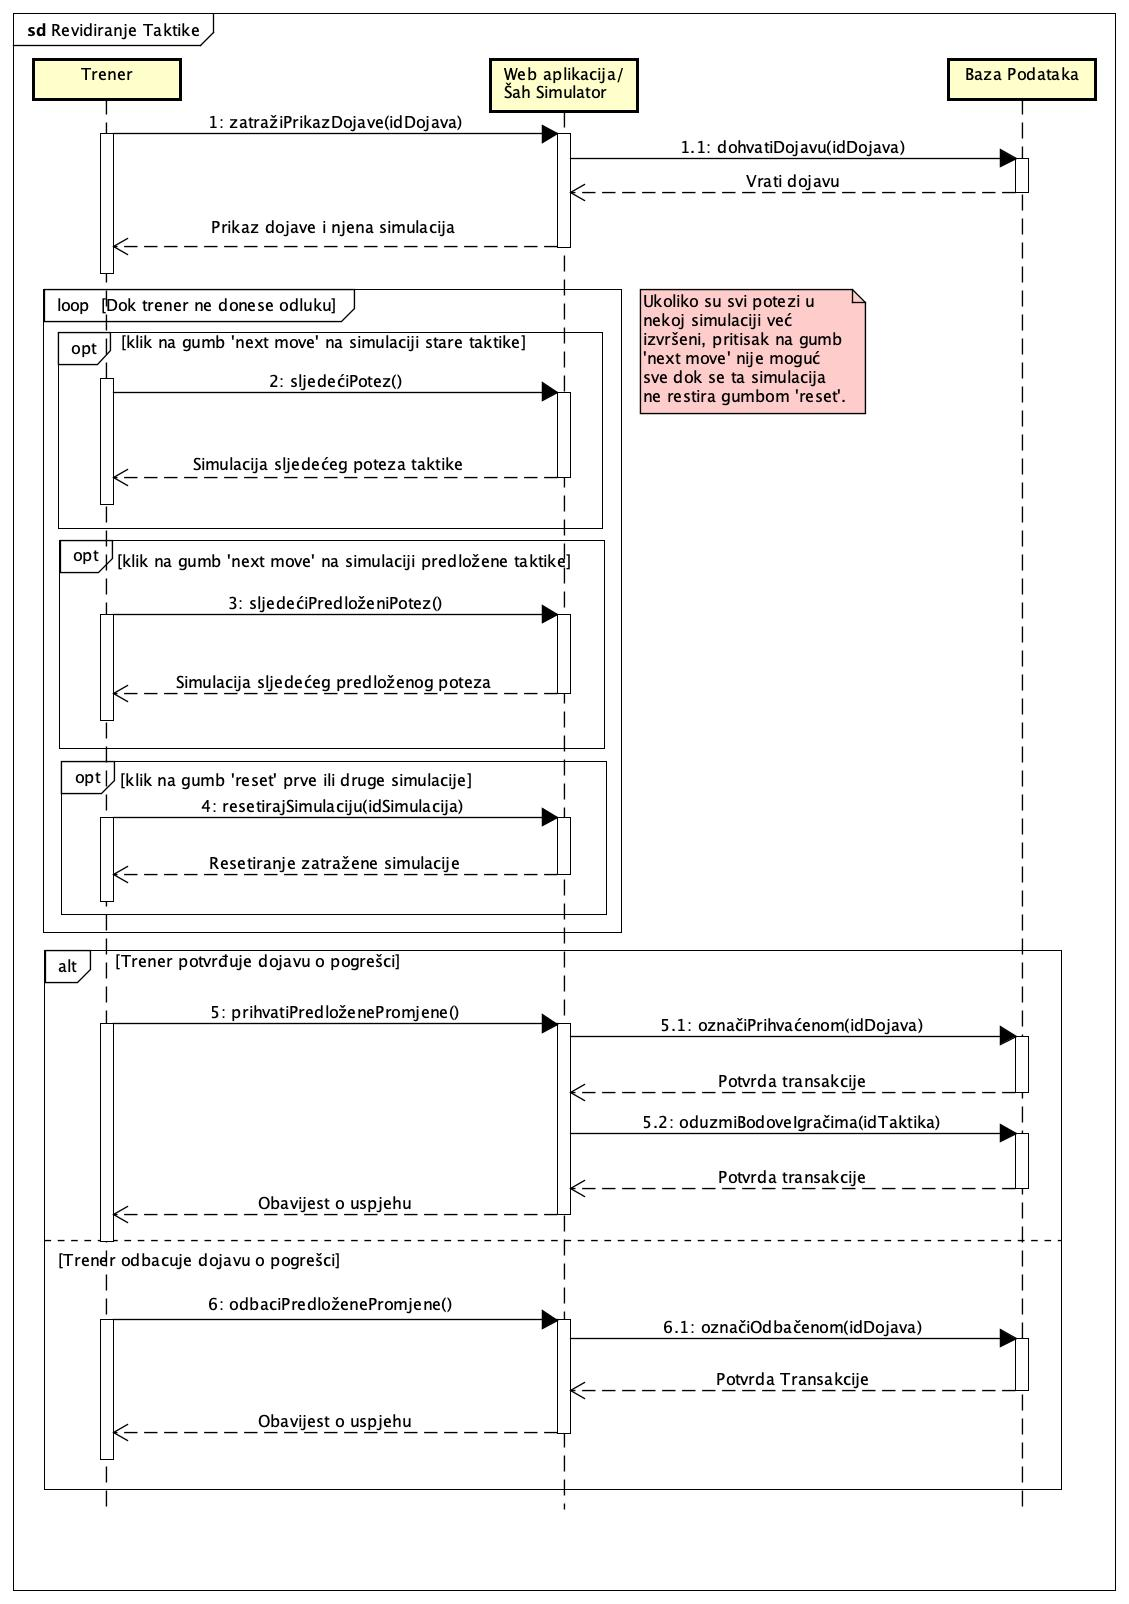
\includegraphics[scale=0.40]{dijagrami/RevidiranjeTaktike.jpg} %veličina slike u odnosu na originalnu datoteku i pozicija slike
        					\caption{Sekvencijski dijagram za UC$<$broj obrasca$>$}
        					\label{fig:UC$<$broj obrasca$>$}
				\end{figure}
				
				\eject
	
		\section{Ostali zahtjevi}
		
			\textbf{\textit{dio 1. revizije}}\\
			
			\textit{Nefunkcionalni zahtjevi i zahtjevi domene primjene dopunjuju funkcionalne zahtjeve. Oni opisuju \textbf{kako se sustav treba ponašati} i koja \textbf{ograničenja} treba poštivati (performanse, korisničko iskustvo, pouzdanost, standardi kvalitete, sigurnost...). Primjeri takvih zahtjeva u Vašem projektu mogu biti: podržani jezici korisničkog sučelja, vrijeme odziva, najveći mogući podržani broj korisnika, podržane web/mobilne platforme, razina zaštite (protokoli komunikacije, kriptiranje...)... Svaki takav zahtjev potrebno je navesti u jednoj ili dvije rečenice.}
			
			Sustav mora osigurati da odgovor na svaki zahtjev dođe unutar 5 sekundi. Sustav mora isto tako osiguravati da korisnici imaju sigurne šifre za svoje korisničke račune kako bi što bolje poboljšao sigurnost sustava. Sustav mora osigurati da svaka osoba ima samo jednu ulogu u aplikaciji. Sustav mora osigurati da korisnici ne mogu raditi ilegalne poteze u šahu.\\
			Sustav mora osigurati da korisnik mora unijeti sve potrebne podatke. \\
			Treneri prilikom stvaranja novog turnira mora unijeti naziv, datum i vrijeme početka te opis turnira. Treneri prilikom stvaranja novog termina treninga ne smije unijeti vrijeme koje mu je već zauzeto drugim terminom. Trener prilikom unosa nove novosti mora osigurati da novost ima naslov i sadržaj. \\
			Administrator prilikom stvaranja novog turnira mora unijeti naziv, datum i vrijeme početka, opis turnira te mora navesti trenera kojeg će sustav prepoznati kao organizatora turnira, pošto će tom treneru biti dane organizatorske ovlasti nad turnirom. Administrator prilikom stvaranja novog termina treninga mora navesti trenera kojem stvara termin te ne smije unijeti vrijeme koje je tom treneru već zauzeto drugim terminom.\\
			Član mora prilikom prijave pogreške u dnevnoj taktici mora unijeti poteze koje smatra ispravnim te opis tih poteza.\\
			Sustav mora mjeriti svakom članu vrijeme potrebno za rješavanje dnevne taktike te koristeći izmjereno vrijeme i ocjenu težine taktike dodijeliti članu bodove za tu taktiku. Sustav na bazi zbroja svih bodova, kreira težinsku listu rang listu članova.\\
			Korisničko sučelje će podržavati samo engleski jezik. Korisničko sučelje mora biti intuitivno za korištenje.\\
			
		 
			 
			 
			 
			 
	
	\chapter{Arhitektura i dizajn sustava}
		
		\textbf{\textit{dio 1. revizije}}\\

		\textit{ Potrebno je opisati stil arhitekture te identificirati: podsustave, preslikavanje na radnu platformu, spremišta podataka, mrežne protokole, globalni upravljački tok i sklopovsko-programske zahtjeve. Po točkama razraditi i popratiti odgovarajućim skicama:}
	\begin{itemize}
		\item 	\textit{izbor arhitekture temeljem principa oblikovanja pokazanih na predavanjima (objasniti zašto ste baš odabrali takvu arhitekturu)}
		\item 	\textit{organizaciju sustava s najviše razine apstrakcije (npr. klijent-poslužitelj, baza podataka, datotečni sustav, grafičko sučelje)}
		\item 	\textit{organizaciju aplikacije (npr. slojevi frontend i backend, MVC arhitektura) }		
	\end{itemize}

	
		

		

				
		\section{Baza podataka}
			
			\textbf{\textit{dio 1. revizije}}\\
			
		\textit{Potrebno je opisati koju vrstu i implementaciju baze podataka ste odabrali, glavne komponente od kojih se sastoji i slično.}
		
			\subsection{Opis tablica}
			

				\textit{Svaku tablicu je potrebno opisati po zadanom predlošku. Lijevo se nalazi točno ime varijable u bazi podataka, u sredini se nalazi tip podataka, a desno se nalazi opis varijable. Svjetlozelenom bojom označite primarni ključ. Svjetlo plavom označite strani ključ}
				
				\begin{longtabu} to \textwidth {|X[6, l]|X[6, l]|X[20, l]|}
					
					\hline \multicolumn{3}{|c|}{\textbf{korisnik - ime tablice}}	 \\[3pt] \hline
					\endfirsthead
					
					\hline \multicolumn{3}{|c|}{\textbf{korisnik - ime tablice}}	 \\[3pt] \hline
					\endhead
					
					\hline 
					\endlastfoot
					
					\cellcolor{LightGreen}IDKorisnik & INT	&  	Lorem ipsum dolor sit amet, consectetur adipiscing elit, sed do eiusmod tempor incididunt ut labore et dolore magna aliqua. Ut enim ad minim veniam 	\\ \hline
					korisnickoIme	& VARCHAR &   	\\ \hline 
					email & VARCHAR &   \\ \hline 
					ime & VARCHAR	&  		\\ \hline 
					\cellcolor{LightBlue} primjer	& VARCHAR &   	\\ \hline 
					
					
				\end{longtabu}
			
			
			\subsection{Dijagram baze podataka}
				\textit{ U ovom potpoglavlju potrebno je umetnuti dijagram baze podataka. Primarni i strani ključevi moraju biti označeni, a tablice povezane. Bazu podataka je potrebno normalizirati. Podsjetite se kolegija "Baze podataka".}
			
			\eject
			
			
		\section{Dijagram razreda}
			\text{Dijagram modela potrebnih za funkcionalnosti autentikacije.}
			\begin{figure}[H]
					\centerfloat
					\advance\leftskip0.7cm
        					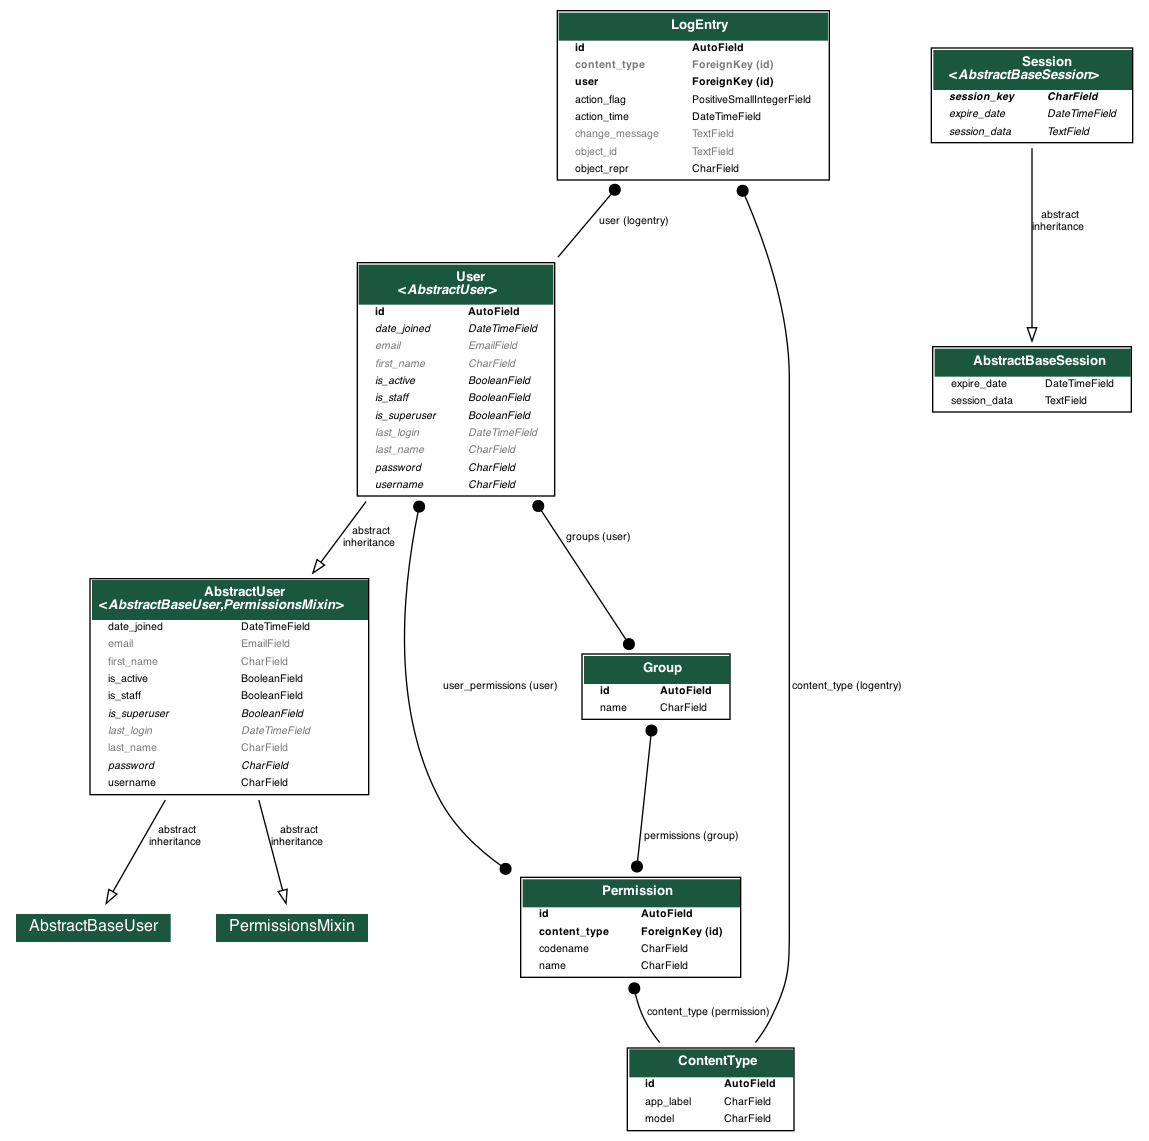
\includegraphics[scale=0.45]{dijagrami/ModelsClassDiagram1.png} %veličina slike u odnosu na originalnu datoteku i pozicija slike
        					\caption{Dijagram razreda modela generične funkcionalnosti}
        					\label{fig:DijagramRazredaModel}
			\end{figure}
			
			\begin{figure}[H]
					\centerfloat
					\advance\leftskip0.7cm
        					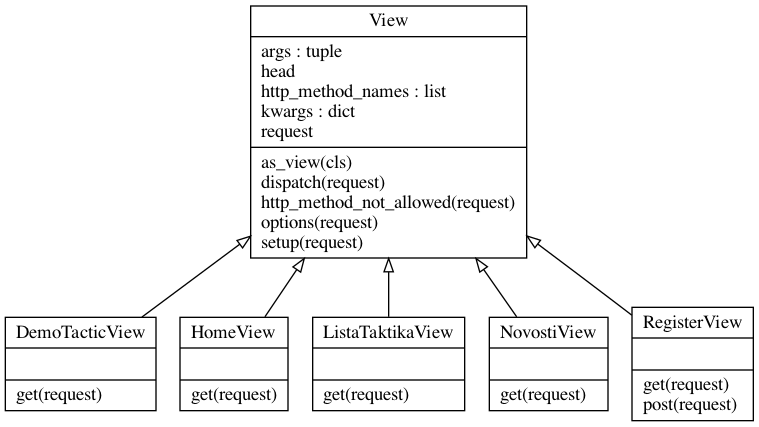
\includegraphics[scale=0.65]{dijagrami/ViewClassDiagram1.png} %veličina slike u odnosu na originalnu datoteku i pozicija slike
        					\caption{Dijagram razreda view-ova generične funkcionalnosti}
        					\label{fig:DijagramRazredaView}
			\end{figure}
			
			\eject
			
			\begin{figure}[H]
					\centerfloat
					\advance\leftskip0.7cm
        					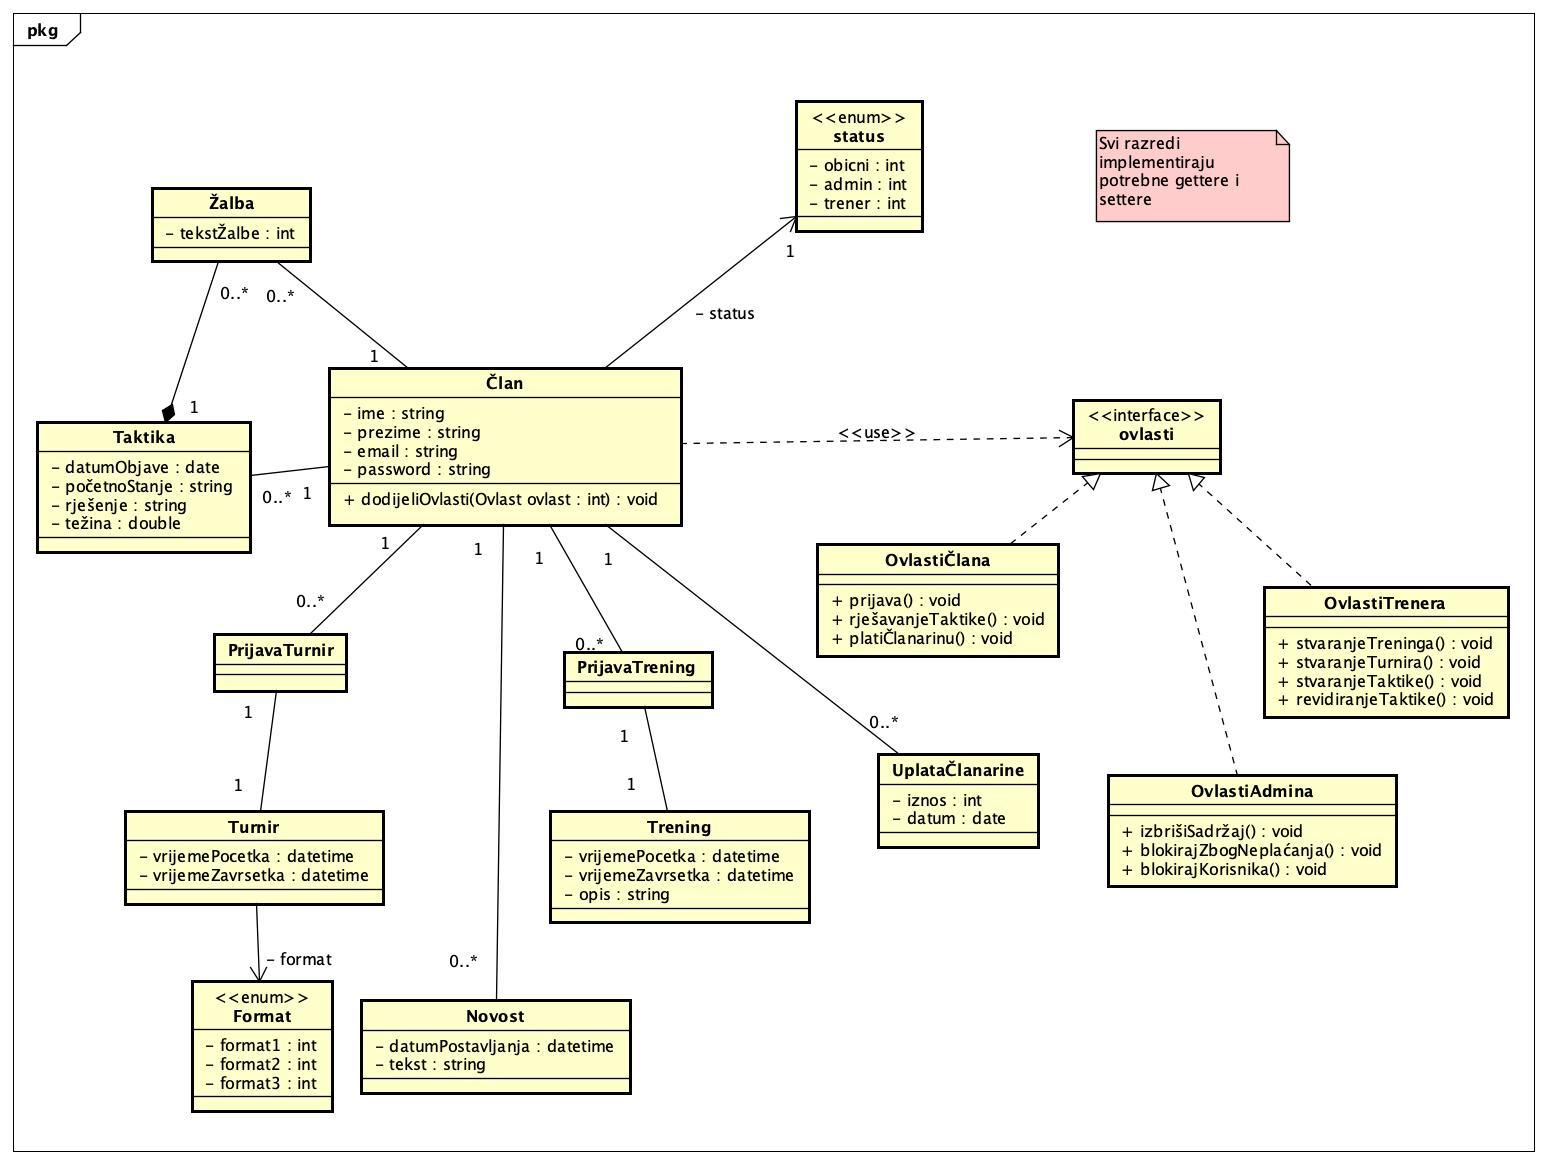
\includegraphics[scale=0.35]{dijagrami/Classdiagram.jpg} %veličina slike u odnosu na originalnu datoteku i pozicija slike
        					\caption{Idejni dijagram razreda}
        					\label{fig:idejniDijagramRazreda}
				\end{figure}

			
			\textbf{\textit{dio 2. revizije}}\\			
			
			\textit{Prilikom druge predaje projekta dijagram razreda i opisi moraju odgovarati stvarnom stanju implementacije}
			
			
			
			\eject
		
		\section{Dijagram stanja}
			
			
			\textbf{\textit{dio 2. revizije}}\\
			
			\textit{Potrebno je priložiti dijagram stanja i opisati ga. Dovoljan je jedan dijagram stanja koji prikazuje \textbf{značajan dio funkcionalnosti} sustava. Na primjer, stanja korisničkog sučelja i tijek korištenja neke ključne funkcionalnosti jesu značajan dio sustava, a registracija i prijava nisu. }
			
			
			\eject 
		
		\section{Dijagram aktivnosti}
			
			\textbf{\textit{dio 2. revizije}}\\
			
			 \textit{Potrebno je priložiti dijagram aktivnosti s pripadajućim opisom. Dijagram aktivnosti treba prikazivati značajan dio sustava.}
			
			\eject
		\section{Dijagram komponenti}
		
			\textbf{\textit{dio 2. revizije}}\\
		
			 \textit{Potrebno je priložiti dijagram komponenti s pripadajućim opisom. Dijagram komponenti treba prikazivati strukturu cijele aplikacije.}
%	\chapter{Implementacija i korisničko sučelje}
		
		
		\section{Korištene tehnologije i alati}
		
			\textbf{\textit{dio 2. revizije}}
			
			 \textit{Detaljno navesti sve tehnologije i alate koji su primijenjeni pri izradi dokumentacije i aplikacije. Ukratko ih opisati, te navesti njihovo značenje i mjesto primjene. Za svaki navedeni alat i tehnologiju je potrebno \textbf{navesti internet poveznicu} gdje se mogu preuzeti ili više saznati o njima}.
			
			
			\eject 
		
	
		\section{Ispitivanje programskog rješenja}
			
			\textbf{\textit{dio 2. revizije}}\\
			
			 \textit{U ovom poglavlju je potrebno opisati provedbu ispitivanja implementiranih funkcionalnosti na razini komponenti i na razini cijelog sustava s prikazom odabranih ispitnih slučajeva. Studenti trebaju ispitati temeljnu funkcionalnost i rubne uvjete.}
	
			
			\subsection{Ispitivanje komponenti}
			\textit{Potrebno je provesti ispitivanje jedinica (engl. unit testing) nad razredima koji implementiraju temeljne funkcionalnosti. Razraditi \textbf{minimalno 6 ispitnih slučajeva} u kojima će se ispitati redovni slučajevi, rubni uvjeti te izazivanje pogreške (engl. exception throwing). Poželjno je stvoriti i ispitni slučaj koji koristi funkcionalnosti koje nisu implementirane. Potrebno je priložiti izvorni kôd svih ispitnih slučajeva te prikaz rezultata izvođenja ispita u razvojnom okruženju (prolaz/pad ispita). }
			
			
			
			\subsection{Ispitivanje sustava}
			
			 \textit{Potrebno je provesti i opisati ispitivanje sustava koristeći radni okvir Selenium\footnote{\url{https://www.seleniumhq.org/}}. Razraditi \textbf{minimalno 4 ispitna slučaja} u kojima će se ispitati redovni slučajevi, rubni uvjeti te poziv funkcionalnosti koja nije implementirana/izaziva pogrešku kako bi se vidjelo na koji način sustav reagira kada nešto nije u potpunosti ostvareno. Ispitni slučaj se treba sastojati od ulaza (npr. korisničko ime i lozinka), očekivanog izlaza ili rezultata, koraka ispitivanja i dobivenog izlaza ili rezultata.\\ }
			 
			 \textit{Izradu ispitnih slučajeva pomoću radnog okvira Selenium moguće je provesti pomoću jednog od sljedeća dva alata:}
			 \begin{itemize}
			 	\item \textit{dodatak za preglednik \textbf{Selenium IDE} - snimanje korisnikovih akcija radi automatskog ponavljanja ispita	}
			 	\item \textit{\textbf{Selenium WebDriver} - podrška za pisanje ispita u jezicima Java, C\#, PHP koristeći posebno programsko sučelje.}
			 \end{itemize}
		 	\textit{Detalji o korištenju alata Selenium bit će prikazani na posebnom predavanju tijekom semestra.}
			
			\eject 
		
		
		\section{Dijagram razmještaja}
			
			\textbf{\textit{dio 2. revizije}}
			
			 \textit{Potrebno je umetnuti \textbf{specifikacijski} dijagram razmještaja i opisati ga. Moguće je umjesto specifikacijskog dijagrama razmještaja umetnuti dijagram razmještaja instanci, pod uvjetom da taj dijagram bolje opisuje neki važniji dio sustava.}
			
			\eject 
		
		\section{Upute za puštanje u pogon}
		
			\textbf{\textit{dio 2. revizije}}\\
		
			 \textit{U ovom poglavlju potrebno je dati upute za puštanje u pogon (engl. deployment) ostvarene aplikacije. Na primjer, za web aplikacije, opisati postupak kojim se od izvornog kôda dolazi do potpuno postavljene baze podataka i poslužitelja koji odgovara na upite korisnika. Za mobilnu aplikaciju, postupak kojim se aplikacija izgradi, te postavi na neku od trgovina. Za stolnu (engl. desktop) aplikaciju, postupak kojim se aplikacija instalira na računalo. Ukoliko mobilne i stolne aplikacije komuniciraju s poslužiteljem i/ili bazom podataka, opisati i postupak njihovog postavljanja. Pri izradi uputa preporučuje se \textbf{naglasiti korake instalacije uporabom natuknica} te koristiti što je više moguće \textbf{slike ekrana} (engl. screenshots) kako bi upute bile jasne i jednostavne za slijediti.}
			
			
			 \textit{Dovršenu aplikaciju potrebno je pokrenuti na javno dostupnom poslužitelju. Studentima se preporuča korištenje neke od sljedećih besplatnih usluga: \href{https://aws.amazon.com/}{Amazon AWS}, \href{https://azure.microsoft.com/en-us/}{Microsoft Azure} ili \href{https://www.heroku.com/}{Heroku}. Mobilne aplikacije trebaju biti objavljene na F-Droid, Google Play ili Amazon App trgovini.}
			
			
			\eject 
%	\chapter{Zaključak i budući rad}
		
		\textbf{\textit{dio 2. revizije}}\\
		
		 \textit{U ovom poglavlju potrebno je napisati osvrt na vrijeme izrade projektnog zadatka, koji su tehnički izazovi prepoznati, jesu li riješeni ili kako bi mogli biti riješeni, koja su znanja stečena pri izradi projekta, koja bi znanja bila posebno potrebna za brže i kvalitetnije ostvarenje projekta i koje bi bile perspektive za nastavak rada u projektnoj grupi.}
		
		 \textit{Potrebno je točno popisati funkcionalnosti koje nisu implementirane u ostvarenoj aplikaciji.}
		
		\eject 
	\chapter*{Popis literature}
		\addcontentsline{toc}{chapter}{Popis literature}
	 	
 		\textbf{\textit{Kontinuirano osvježavanje}}
	
		\textit{Popisati sve reference i literaturu koja je pomogla pri ostvarivanju projekta.}
		
		
		\begin{enumerate}
			
			
			\item  Programsko inženjerstvo, FER ZEMRIS, \url{http://www.fer.hr/predmet/proinz}
			
			\item  I. Sommerville, "Software engineering", 8th ed, Addison Wesley, 2007.
			
			\item  T.C.Lethbridge, R.Langaniere, "Object-Oriented Software Engineering", 2nd ed. McGraw-Hill, 2005.
			
			\item  I. Marsic, Software engineering book``, Department of Electrical and Computer Engineering, Rutgers University, \url{http://www.ece.rutgers.edu/~marsic/books/SE}
			
			\item  The Unified Modeling Language, \url{https://www.uml-diagrams.org/}
			
			\item  Astah Community, \url{http://astah.net/editions/uml-new}
		\end{enumerate}
		
		 
	
	
%	\begingroup
%	\renewcommand*\listfigurename{Indeks slika i dijagrama}
%	%\renewcommand*\listtablename{Indeks tablica}
%	%\let\clearpage\relax
%	\listoffigures
%	%\vspace{10mm}
%	%\listoftables
%	\endgroup
%	\addcontentsline{toc}{chapter}{Indeks slika i dijagrama}


	
	\eject 
		
	%\documentclass[12pt]{report} 
%\begin{document}

\chapter*{Dodatak: Prikaz aktivnosti grupe}
		\addcontentsline{toc}{chapter}{Dodatak: Prikaz aktivnosti grupe}
		
		\section*{Dnevnik sastajanja}
		
		\begin{packed_enum}
			\item  sastanak
			
			\item[] \begin{packed_item}
				\item Datum: 5. listopada 2020. 
				\item Prisustvovali:  Igor Stančin, svi članovi tima
				\item Teme sastanka:
				\begin{packed_item}
					\item  Uvodni sastanak s asistentom
				\end{packed_item}
			\end{packed_item}
			
			\item  sastanak
			\item[] \begin{packed_item}
				\item Datum: 7. listopada 2020. 
				\item Prisustvovali: svi članovi tima
				\item Teme sastanka:
				\begin{packed_item}
					\item  upoznavanje
					\item  dogovor o tehnologijama
				\end{packed_item}
			\end{packed_item}
			
			\item  sastanak
			\item[] \begin{packed_item}
				\item Datum: 12. listopada 2020. 
				\item Prisustvovali: Igor Stančin, Ivan Klabučar, Petar Gabrijel Kedmenec
				\item Teme sastanka:
				\begin{packed_item}
					\item  pitanja oko funkcionalnih zahtjeva
				\end{packed_item}
			\end{packed_item}
			
			\item  sastanak
			\item[] \begin{packed_item}
				\item Datum: 15. listopada 2020. 
				\item Prisustvovali: svi članovi tima
				\item Teme sastanka:
				\begin{packed_item}
					\item  raspodjela poslova oko obrazaca uporabe
				\end{packed_item}
			\end{packed_item}
			
			\item  sastanak
			\item[] \begin{packed_item}
				\item Datum: 21. listopada 2020. 
				\item Prisustvovali: svi članovi tima
				\item Teme sastanka:
				\begin{packed_item}
					\item  raspodjela poslova oko UML dijagrama
					\item  rasprava o prirodi uloge Admin
				\end{packed_item}
			\end{packed_item}
		
			\item  sastanak
			\item[] \begin{packed_item}
				\item Datum: 24. listopada 2020. 
				\item Prisustvovali: Ivan Klabučar, Fran Leontić, Luka Žižić
				\item Teme sastanka:
				\begin{packed_item}
					\item  raspravljanje o implementaciji dnevnih taktika
				\end{packed_item}
			\end{packed_item}
			
			\item  sastanak
			\item[] \begin{packed_item}
				\item Datum: 24. listopada 2020. 
				\item Prisustvovali: Ivan Klabučar, Petar Gabrijel Kedmenec
				\item Teme sastanka:
				\begin{packed_item}
					\item  rješavanje konflikata na GitLabu
				\end{packed_item}
			\end{packed_item}
		
			\item  sastanak
			\item[] \begin{packed_item}
				\item Datum: 26. listopada 2020. 
				\item Prisustvovali: Igor Stančin, svi članovi tima
				\item Teme sastanka:
				\begin{packed_item}
					\item  razjašnjavanje dijagrama obrazaca i sekvencijskih dijagrama
				\end{packed_item}
			\end{packed_item}
			
			\item  sastanak
			\item[] \begin{packed_item}
				\item Datum: 29. listopada 2020. 
				\item Prisustvovali: svi članovi tima
				\item Teme sastanka:
				\begin{packed_item}
					\item  raspodjela kodiranja
				\end{packed_item}
				\item Zaključci:
				\begin{packed_item}
					\item Ivar Cmrečak, Fran Leontić i Ivan Klabučar rade na bazi
					\item Petar Gabrijel Kedmenec i Luka Žižić rade na uspostavljanju templatea za listanje dnevnih taktika
					\item Mihael Svetec i Sven Paprskar rade na uspostavljanju templatea za listanje novosti
				\end{packed_item}
			\end{packed_item}
		
			\item  sastanak
			\item[] \begin{packed_item}
				\item Datum: 31. listopada 2020. 
				\item Prisustvovali: Ivan Klabučar, Fran Leontić, Luka Žižić, Ivar Cmrečak
				\item Teme sastanka:
				\begin{packed_item}
					\item  raspravljanje o tablicama u bazi podataka
				\end{packed_item}
			\end{packed_item}

		\eject 
			\item  sastanak
			\item[] \begin{packed_item}
				\item Datum: 4. studenoga 2020. 
				\item Prisustvovali: svi članovi tima
				\item Teme sastanka:
				\begin{packed_item}
					\item  raspravljanje o implementaciji potrebnih funkcija za demonstraciju generičke funkcionalnosti
				\end{packed_item}
			\end{packed_item}
		
			\item  sastanak
			\item[] \begin{packed_item}
				\item Datum: 9. studenoga 2020. 
				\item Prisustvovali: Igor Stančin, svi članovi tima
				\item Teme sastanka:
				\begin{packed_item}
					\item pokazivanje generičke funkcionalnosti aplikacije
					\item pregled dokumentacije
				\end{packed_item}
			\end{packed_item}
			
			\item  sastanak
			\item[] \begin{packed_item}
				\item Datum: 11. studenoga 2020. 
				\item Prisustvovali: Ivan Klabučar, Ivar Cmrečak, Petar Gabrijel Kedmenec, Fran Leontić, Mihael Svetec, Sven Paprskar
				\item Teme sastanka:
				\begin{packed_item}
					\item raspodjela uloga prije pauze za međuispite
				\end{packed_item}
				\item Zaključci:
				\begin{packed_item}
					\item Petar Gabrijel Kedmenec dovršava uređenje dokumentacije za prvu predaju
					\item Sven Paprskar izrađuje template za prikaz transakcija
					\item Luka Žižić izrađuje template za dodavanje novih obavijesti
					\item Mihael Svetec izrađuje template za dodavanje, listanje i prijavljivanje na treninge
					\item Fran Leontić izrađuje template za prikaz korisničkog profila
					\item Ivan Klabučar izrađuje template za objavu treninga
					\item Ivar Cmrečak uspostavlja bazu podataka
				\end{packed_item}
			\end{packed_item}
			
			\item  sastanak
			\item[] \begin{packed_item}
				\item Datum: 18. studenoga 2020. 
				\item Prisustvovali: svi članovi tima
				\item Teme sastanka:
				\begin{packed_item}
					\item  pregled napravljenog i komentiranje o potrebnim ispravcima programskog koda
				\end{packed_item}
			\end{packed_item}
			\eject
			\item  sastanak
			\item[] \begin{packed_item}
				\item Datum: 25. studenoga 2020. 
				\item Prisustvovali: svi članovi tima
				\item Teme sastanka:
				\begin{packed_item}
					\item  daljnja podjela rada vezana uz kodiranje i dokumentaciju
				\end{packed_item}
			\end{packed_item}
			
			\item  sastanak
			\item[] \begin{packed_item}
				\item Datum: 2. prosinca 2020. 
				\item Prisustvovali: svi članovi tima
				\item Teme sastanka:
				\begin{packed_item}
					\item  razrješavanje problema vezanog uz programiranje
				\end{packed_item}
			\end{packed_item}
			
			\item  sastanak
			\item[] \begin{packed_item}
				\item Datum: 9. prosinca 2020. 
				\item Prisustvovali: svi članovi tima
				\item Teme sastanka:
				\begin{packed_item}
					\item  analiza dosadašnjeg rada, dogovor o nastavku rada
				\end{packed_item}
			\end{packed_item}
			
			\item  sastanak
			\item[] \begin{packed_item}
				\item Datum: 14. prosinca 2020. 
				\item Prisustvovali: svi članovi tima
				\item Teme sastanka:
				\begin{packed_item}
					\item  dokumentacija, raspravljanje parova koji rade na zajedničkom problemu
				\end{packed_item}
			\end{packed_item}
			
			\item  sastanak
			\item[] \begin{packed_item}
				\item Datum: 18. prosinca 2020. 
				\item Prisustvovali: svi članovi tima
				\item Teme sastanka:
				\begin{packed_item}
					\item  dogovor o nastavku rada na dokumentaciji i programskim rješenjima
				\end{packed_item}
			\end{packed_item}
			
			\item  sastanak
			\item[] \begin{packed_item}
				\item Datum: 23. prosinca 2020. 
				\item Prisustvovali: svi članovi tima
				\item Teme sastanka:
				\begin{packed_item}
					\item  podjela posla preko zimskih praznika
				\end{packed_item}
			\end{packed_item}
		
		\item  sastanak
		\item[] \begin{packed_item}
			\item Datum: 4. siječnja 2021. 
			\item Prisustvovali: svi članovi tima
			\item Teme sastanka:
			\begin{packed_item}
				\item dogovori oko završavanja programiranja vezanog uz alfa verziju aplikacije
			\end{packed_item}
		\end{packed_item}
			
			\item  sastanak
			\item[] \begin{packed_item}
				\item Datum: 4. siječnja 2021. 
				\item Prisustvovali: Igor Stančin, svi članovi tima
				\item Teme sastanka:
				\begin{packed_item}
					\item prezentacija alfa inačice aplikacije asistentu Igoru Stančinu
				\end{packed_item}
			\end{packed_item}
		\end{packed_enum}
		
		\eject
		\section*{Tablica aktivnosti}
		
			\textbf{\textit{Kontinuirano osvježavanje}}\\
			
			 \textit{Napomena: Doprinose u aktivnostima treba navesti u satima po članovima grupe po aktivnosti.}
					
						
			
			\begin{longtabu} to \textwidth {|X[7, l]|X[1, c]|X[1, c]|X[1, c]|X[1, c]|X[1, c]|X[1, c]|X[1, c]|}
								
				\cline{2-8} \multicolumn{1}{c|}{\textbf{}} &     \multicolumn{1}{c|}{\rotatebox{90}{\textbf{Ivar Cmrečak}}} & \multicolumn{1}{c|}{\rotatebox{90}{\textbf{Sven Paprskar }}} &	\multicolumn{1}{c|}{\rotatebox{90}{\textbf{Ivan Klabučar}}} &	\multicolumn{1}{c|}{\rotatebox{90}{\textbf{Mihael Svetec }}} &
				\multicolumn{1}{c|}{\rotatebox{90}{\textbf{Fran Leontić }}} &
				\multicolumn{1}{c|}{\rotatebox{90}{\textbf{Petar Gabrijel Kedmenec }}} &	\multicolumn{1}{c|}{\rotatebox{90}{\textbf{Luka Žižić }}} \\ \hline 
				\endfirsthead
				
			
				\cline{2-8} \multicolumn{1}{c|}{\textbf{}} &     \multicolumn{1}{c|}{\rotatebox{90}{\textbf{Ivar Cmrečak}}} & \multicolumn{1}{c|}{\rotatebox{90}{\textbf{Sven Paprskar }}} &	\multicolumn{1}{c|}{\rotatebox{90}{\textbf{Ivan Klabučar}}} &
				\multicolumn{1}{c|}{\rotatebox{90}{\textbf{Mihael Svetec }}} &	\multicolumn{1}{c|}{\rotatebox{90}{\textbf{Fran Leontić }}} &
				\multicolumn{1}{c|}{\rotatebox{90}{\textbf{Petar Gabrijel Kedmenec }}} &	\multicolumn{1}{c|}{\rotatebox{90}{\textbf{Luka Žižić }}} \\ \hline 
				\endhead
				
				
				\endfoot
							
				 
				\endlastfoot
				
				Upravljanje projektom 		& 10 &  & 12 &  &  &  & \\ \hline
				Opis projektnog zadatka 	&  & 1 & 1 &  & 2.5  &  & 2\\ \hline
				
				Funkcionalni zahtjevi       &  & 1 &  &  &  & 3 &  \\ \hline
				Opis pojedinih obrazaca 	& 1 & 2 & 1 & 3 &  & 3 & \\ \hline
				Dijagram obrazaca 			&  & 1 &  & 2 &  &  & \\ \hline
				Sekvencijski dijagrami 		&  &  & 3 &  & 1.5 &  & 2.5\\ \hline
				Opis ostalih zahtjeva 		&  &  &  &  &  & 1.5 &  \\ \hline

				Arhitektura i dizajn sustava	 & 1 &  &  &  &  &  &  \\ \hline
				Baza podataka				& 1 &  & 2 & 1 & 2 & 1 & 1 \\ \hline
				Dijagram razreda 			&  &  & 5 &  & 1 &  &   \\ \hline
				Dijagram stanja				&  & 5 &  &  &  &  &  \\ \hline
				Dijagram aktivnosti 		&  & 2 &  &  &  &  &  \\ \hline
				Dijagram komponenti			&  &  &  &  &  &  &  \\ \hline
				Korištene tehnologije i alati 		& 2 & 2 &  &  &  &  &  \\ \hline
				Ispitivanje programskog rješenja 	&  & 2 & 1 & 1 &  &  &  \\ \hline
				Dijagram razmještaja			&  & 1.5 &  &  &  &  &  \\ \hline
				Upute za puštanje u pogon 		&  & 1.5 &  &  &  &  &  \\ \hline 
				Dnevnik sastajanja 			&  & 1 & .5 &  &  & 1 &  \\ \hline
				Zaključak i budući rad 		&  & 1 &  &  &  &  &  \\  \hline
				Popis literature 			&  &  &  &  &  & .5 &  \\  \hline
				&  &  &  &  &  &  &  \\ \hline \hline
				Izrada baze podataka 		& 3 &  & 3 &  &  &  & \\ \hline 
				Spajanje s bazom podataka 		& 3 &  &  &  &  &  &  \\ \hline
				Izrada frontenda 			& 3 &  & 6 &  & 2  &  &  \\  \hline
				Izrada autorizacije 			& 3 &  &  &  &  &  & \\  \hline
				Izrada stranice s novostima 			&  & 2 &  & 2 &  &  & 5 \\  \hline
				Izrada stranice s dnevnim taktikama 		&  &  & 6 &  &  & 2 & 3 \\  \hline
				Izrada stranice s treninzima 		&  &  &  & 5 &  &  &  \\ \hline
				Izrada stranice s turnirima 		&  &  &  & 5 &  &  &  \\ \hline
				Izrada početne stranice i nav-bara 		&  &  &  & 2 &  &  & 0.5 \\ \hline
				Izrada stranice s dojavama pogreški 		&  &  &  & 3 &  &  &  \\ \hline
				Izrada stranice profila		&  &  &  &  & 5 &  &  \\ \hline
				Izrada liste profila i detaljnog prikaza		&  &  &  &  & 4 &  &  \\ \hline
				Izrada stranice za plaćanje članarine 		&  &  &  &  &  &  & 3 \\ \hline
				Izrada adminove liste neplaćenh članarina		&  &  &  &  & 2 & 1 &  \\ \hline
				Izrada adminove liste svih transakcija &  &  &  &  &  & 4 &  \\ \hline
				Izrada rang liste &  &  & 3 &  &  & 1 &  \\ \hline
				Deployment na remote server & 4 &  &  &  &  &  &  \\ \hline
				
			\end{longtabu}
					
					
		\eject
		\section*{Dijagrami pregleda promjena}
		
		\textbf{\textit{dio 2. revizije}}\\
		
		\textit{Prenijeti dijagram pregleda promjena nad datotekama projekta. Potrebno je na kraju projekta generirane grafove s gitlaba prenijeti u ovo poglavlje dokumentacije. Dijagrami za vlastiti projekt se mogu preuzeti s gitlab.com stranice, u izborniku Repository, pritiskom na stavku Contributors.}
		
	\end{document}


\end{document} %naredbe i tekst nakon ove naredbe ne ulaze u izgrađen dokument 


